\documentclass[a4paper, abstract=on]{scrreprt}
\usepackage[utf8]{inputenc}
\usepackage[T1]{fontenc}
\usepackage{geometry}
\usepackage{csquotes}
\usepackage[english]{babel}
\usepackage{float}
\usepackage{ulem}
\usepackage{lastpage}
\usepackage{blindtext}
\usepackage{tikz}
\usepackage{graphicx}
\usepackage{tabularx}
\usepackage{hyperref}
\usepackage[backend=bibtex,style=ieee]{biblatex}
\usepackage{enumitem}
\usepackage[color=red!100!green!33]{todonotes}
\usepackage{pdfpages}
\usepackage{lipsum}
\usepackage{ragged2e}

\addbibresource{doc.bib}
\bibliography{doc}
\graphicspath{{./img/}}

\geometry{a4paper, total={170mm,257mm}, left=20mm, top=20mm}

\title{Title}
\author{Vorname Nachname}
\date{\today}


\begin{document}

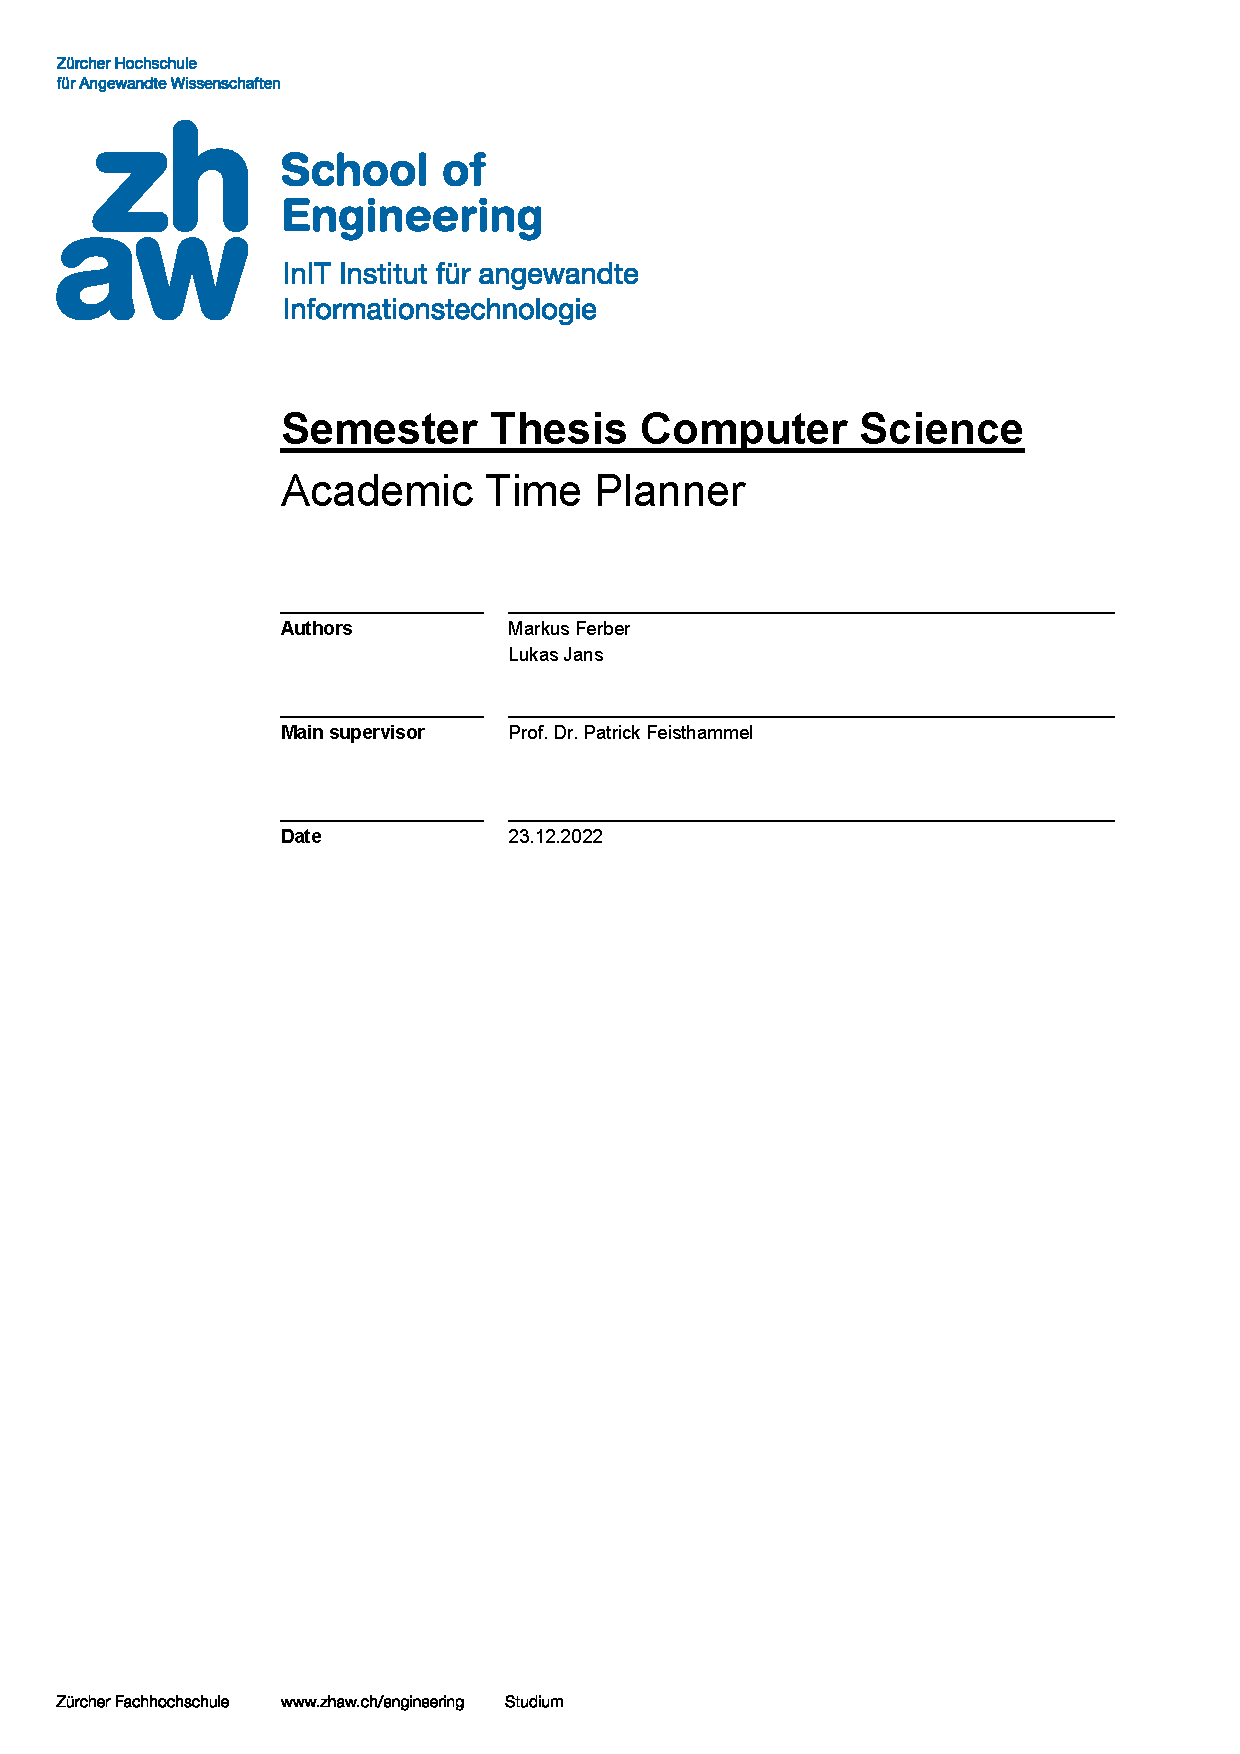
\includepdf{ressources/titlepage}

% Titelseite nicht als erste Seite zählen
\clearpage
\setcounter{page}{1}


\includepdf{ressources/Erklaerung_BA}

\selectlanguage{english} 
\begin{abstract}
%%% Local Variables:
%%% mode: latex
%%% TeX-master: "../doc"
%%% coding: utf-8
%%% End:
% !TEX TS-program = pdflatexmk
% !TEX encoding = UTF-8 Unicode
% !TEX root = ../doc.tex
\lipsum[1]

\end{abstract}

\chapter*{Preface}
%%% Local Variables:
%%% mode: latex
%%% TeX-master: "../doc"
%%% coding: utf-8
%%% End:
% !TEX TS-program = pdflatexmk
% !TEX encoding = UTF-8 Unicode
% !TEX root = ../doc.tex

This semester thesis was written by Markus Ferber and Lukas Jans in the fifth semester of their bachelor's degree in computer science at the Zurich University of Applied Sciences ZHAW in Winterthur. The authors would like to thank their supervisor, Patrick Feisthammel, as well as their additional advisor, Prof. Dr. Karl Rege, for their helpful advice and support throughout the realization of the thesis. They would also like to thank Mrs. Angelika Langham for her review of the thesis and her helpful remarks regarding the use of English language.\\
For the authors, this thesis presented a good opportunity to deepen their knowledge in software development. Many lessons could be learnt, in particular regarding the use of .NET technology and frameworks as well as the Fluxor design pattern.
\thispagestyle{empty}

\tableofcontents
\thispagestyle{empty}


\chapter{Introduction}
\setcounter{page}{1}
%%% Local Variables:
%%% mode: latex
%%% TeX-master: "../doc"
%%% coding: utf-8
%%% End:
% !TEX TS-program = pdflatexmk
% !TEX encoding = UTF-8 Unicode
% !TEX root = ../doc.tex

This section consists of the state of the art and the definition of the project. In the state of the art, the existing software prototype for this project and the approaches used for it are briefly explained. In the definition of project, the tasks and aims of the project are described, based on the definition provided by the supervisor.

\section{Initial position} \label{Initial position}
Toggl Track \cite{toggl_track_url} is an online application frequently used for time planning and tracking for projects or tasks. However, it does not provide the flexibility demanded by teachers and students in order to properly plan, track and compare their time efforts \cite{bachelorarbeit_Egger_Verstappen_page2}. In the bachelor thesis \cite{bachelorarbeit_Egger_Verstappen_page1} on which this project is based, a technological prototype of an academic time planning software (Academic Time Planner, ATP) has been developed. The ATP is designed for complementary use with Toggl Track. The prototype has been realized as a .NET Blazor application fetching time data collected on Toggl Track via the Toggl Track API. Moreover, a concept for mapping Toggl Track time data to ATP-specific time data as well as mockups for the graphical user interface of the ATP have been evaluated.

\section{Definition of project}
Students and teachers have to organise their time for different tasks. The ATP is intended to support them in this matter, allowing for a semester-oriented time planning and helping to keep to the timing plans. To achieve this, the difference between planed time and used time should always be visible. The time tracked is read via an API from Toggl Track (see chapter \ref{Initial position}). The goal of this project is to create a prototype based on the technological prototype already created and to realize the mapping concept, focussing on good and simple usability.

The prototype should be able to run locally and display an overview over the current difference between planed time and used time. To allow for proper handling of time planning data, it should be grouped into plan projects. A plan project contains all time planning data for a certain project (e. g. a semester module). Furthermore, it should include the state of the application as to whether the data fetched from Toggl Track is up-to-date and if there are any inconsistencies between plan projects and Toggle Track projects. In addition to that, the import and export of planning data as well as the creation of plan projects via the application GUI should be made possible.

The following chapters describe the realization of the project. In chapter 2, the fundamentals of the realization are explained. In chapter 3, the methods are described, and in chapter 4 the results. In chapter 5, the results from chapter 4 are discussed and further steps are suggested.
 




\chapter{Fundamentals}
%%% Local Variables:
%%% mode: latex
%%% TeX-master: "../doc"
%%% coding: utf-8
%%% End:
% !TEX TS-program = pdflatexmk
% !TEX encoding = UTF-8 Unicode
% !TEX root = ../doc.tex

This sections explains the fundamental technologies and achievements from previous projects which have been applied in the project.

\section{Technological prototype} \label{Prototype}
As mentioned in chapter \ref{Initial position}, a technological prototype for the ATP has already been developed in a bachelor thesis during the previous semester. The prototype has been realized as a locally running application using the ASP.NET Core Blazor framework and Fluxor for frontend behaviour control \cite{bachelorarbeit_Egger_Verstappen_page4-7}. The application fetches time data from Toggl Track via the Toggl Track API and relies on Local Storage for storing the application state. The graphical user interface has been designed with elements from the Bootstrap toolkit. Charts.js is used to display graphs and charts. The application is made available as a Docker image which can be downloaded from the GitHub Container Registry. As to software testing, unit tests for the part managing the communication between the application and Toggl have been implemented and can be run automatically via GitHub Actions. \cite{bachelorarbeit_Egger_Verstappen_page23-25}.

The different features, however, have not been fully implemented yet. The charts display dummy data instead of real time data, as shown in figure \ref{figure1}. The tracked time data can be retrieved from Toggl, but no further action is applied to it. Local Storage is not considered to be suitable for application data storage on the long term. Further possible enhancements include localization, accessing other APIs and not just Toggl, different installation and update strategies as well as additional automated tests like UI tests and integration tests. \cite{bachelorarbeit_Egger_Verstappen_page26-27}

\begin{figure}[H]
\centering
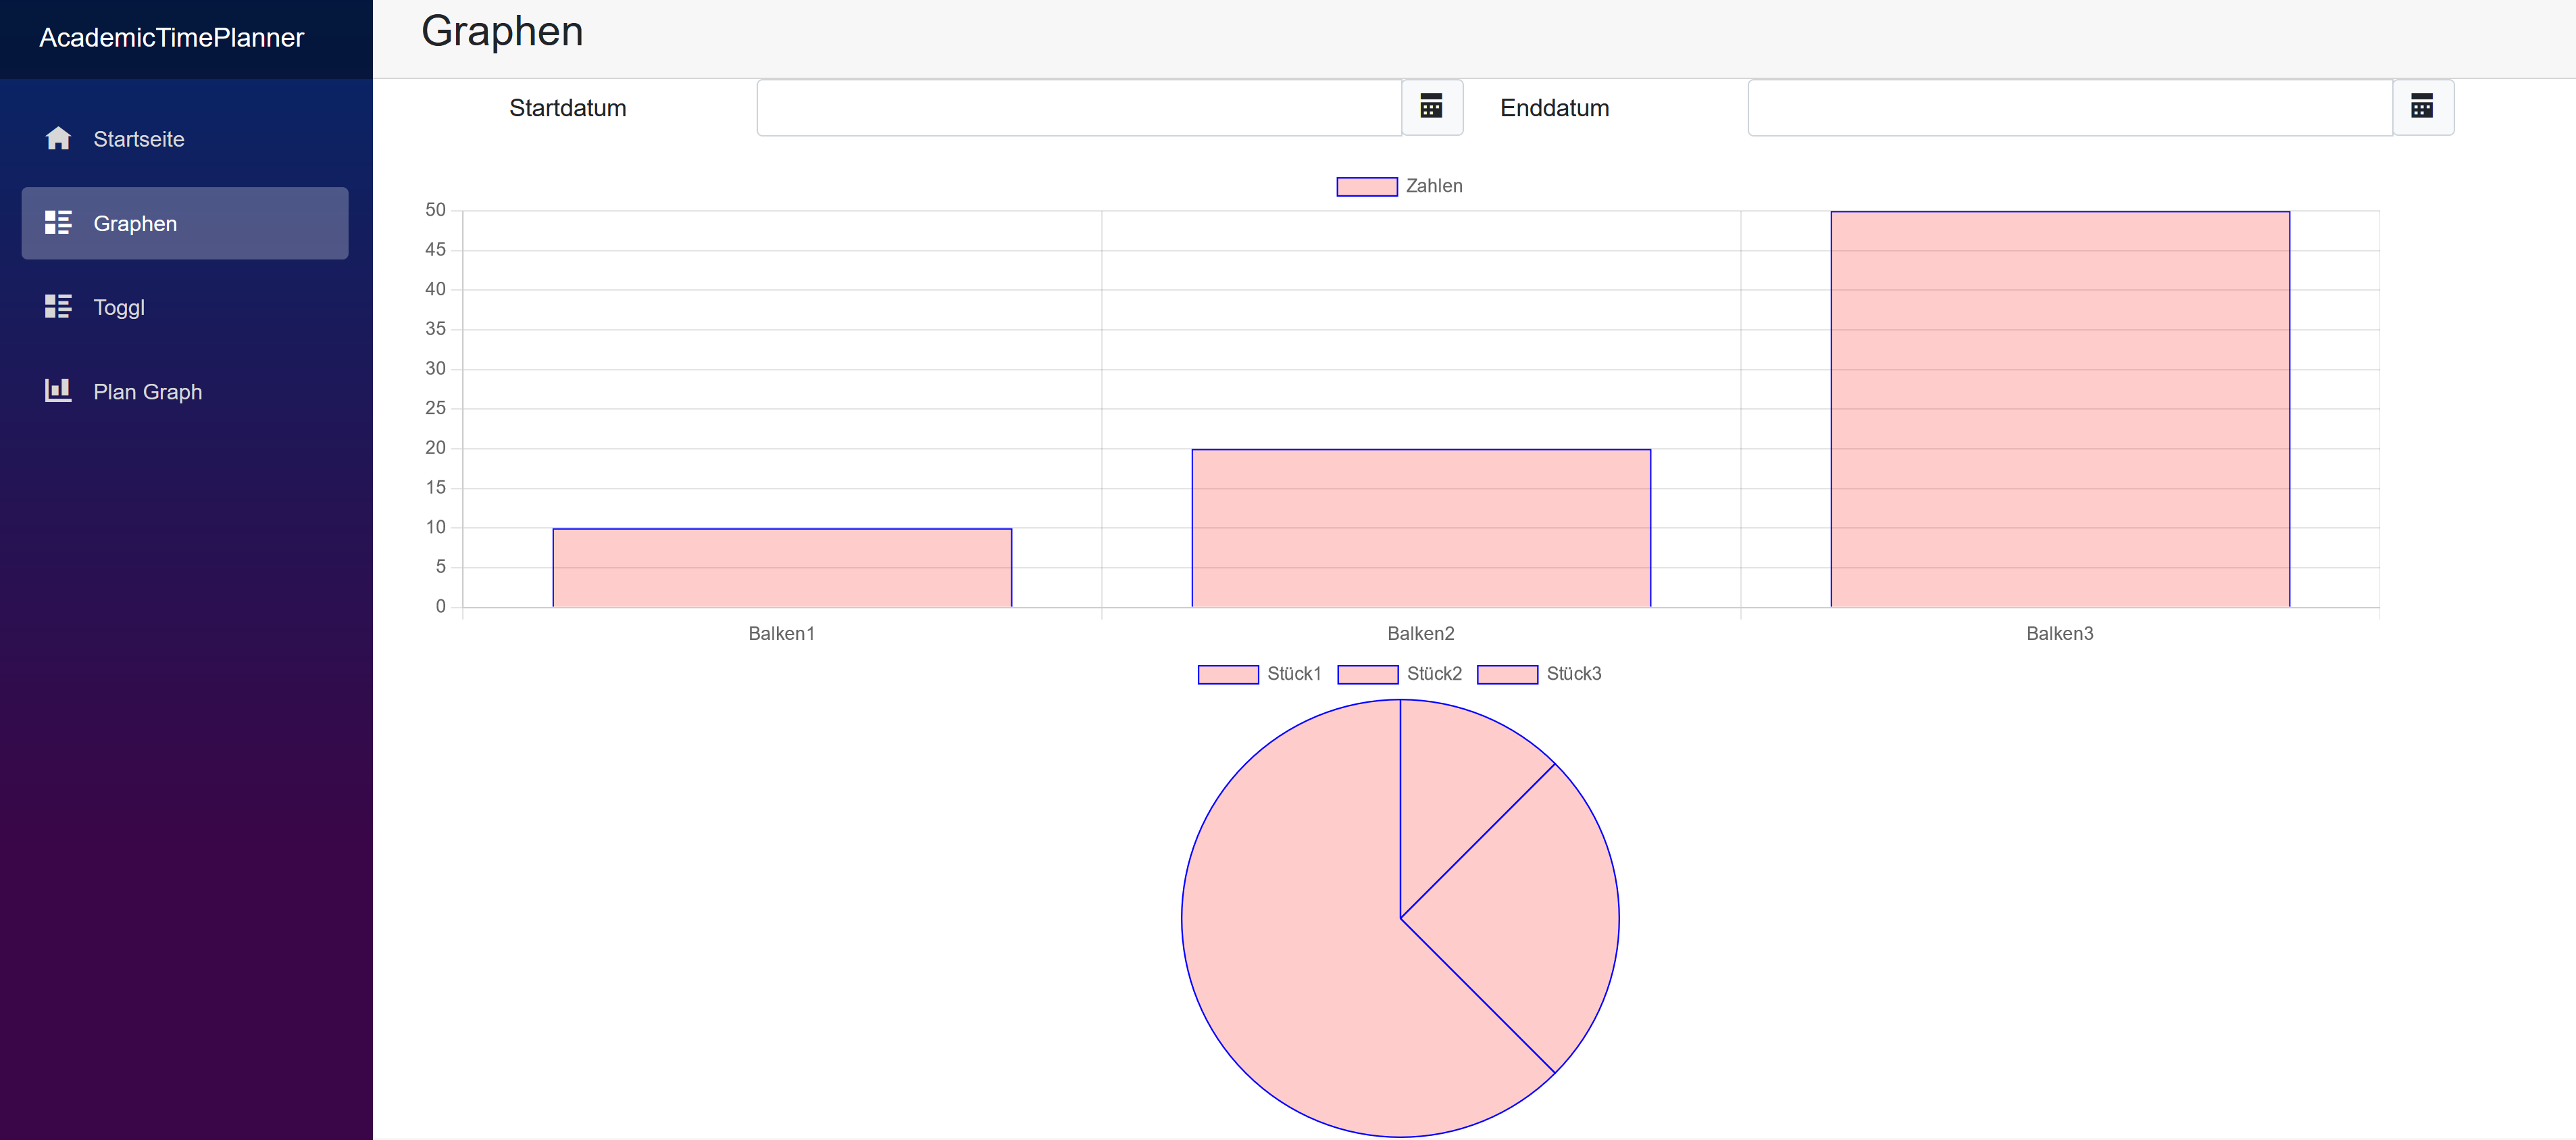
\includegraphics[width=1.0\columnwidth]{figure1_prototype_charts}
\caption{ATP prototype displaying dummy charts}
\label{figure1}
\end{figure}

\section{Toggl Track}
Toggl Track is an easy-to-use, multifunctional online time tracking application. Tasks can be tracked and grouped into projects. Tracking can be started and stopped using start and stop buttons. Times can also be manually entered and assigned to a task and a project. Toggl Track offers many additional functionalities including billing and invoicing, payroll calculating, generation of detailed reports and project budgeting. Toggl Track can be used on different devices like computers, smartphones and tablets. The tracking data is then synchronized between the devices. Furthermore, Toggl Track provides an API to be used to query tracked time entries from Toggl Track which can then be used outside Toggl Track itself, e. g. by other applications. \cite{bachelorarbeit_Egger_Verstappen_page8} \cite{toggl_track_url}

\section{Mapping Concept} \label{Mapping concept}
The mapping concept developed in the aforementioned bachelor thesis \cite{bachelorarbeit_Egger_Verstappen_page20-22} laid the foundation for this project. It determined how the data structure would be built and how the application would interact with Toggl Track. The concept was split into three entities; Plan, Toggl, and Budget and Group. 

\begin{figure}[H]
	\centering
	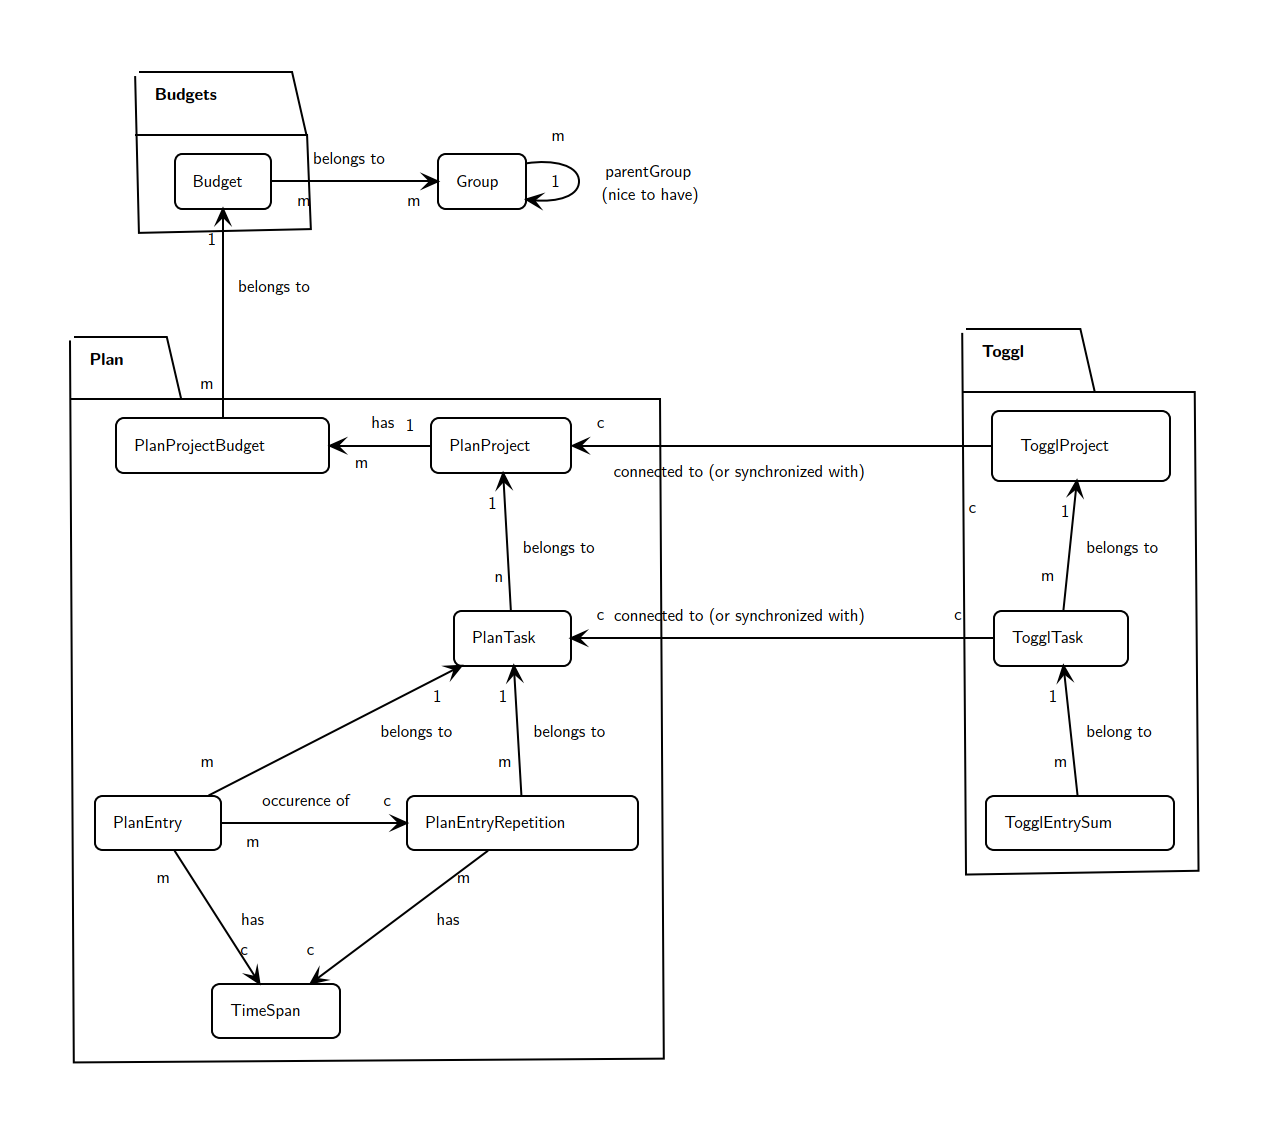
\includegraphics[width=1.0\columnwidth]{entitydiagram_prototype}
	\caption{Entity Relationship Diagram of the bachelor thesis prototype}
	\label{figure2}
\end{figure}

\subsection{Plan}
The plan consists of a plan entry which has a start and an end date as well as a time span. Start and end date denote in which time frame the task is planned, whereby the smallest unit of time is a day. The time span represents the time investment predicted for the task and has a unit of hours. This time span does not have to match the duration between start and end date and can be shorter.
\subsection{Toggl}
To save the data provided by Toggl, three entities are proposed in the bachelor thesis. Those entities save only the data needed by the ATP. They have an attribute togglId which corresponds with the ID given by Toggl. To compare the data of the plan project or the plan task with the tracked time, TogglProject and TogglTask were defined. The time captured in Toggl can be saved in the TogglEntrySum.

\begin{figure}[H]
	\centering
	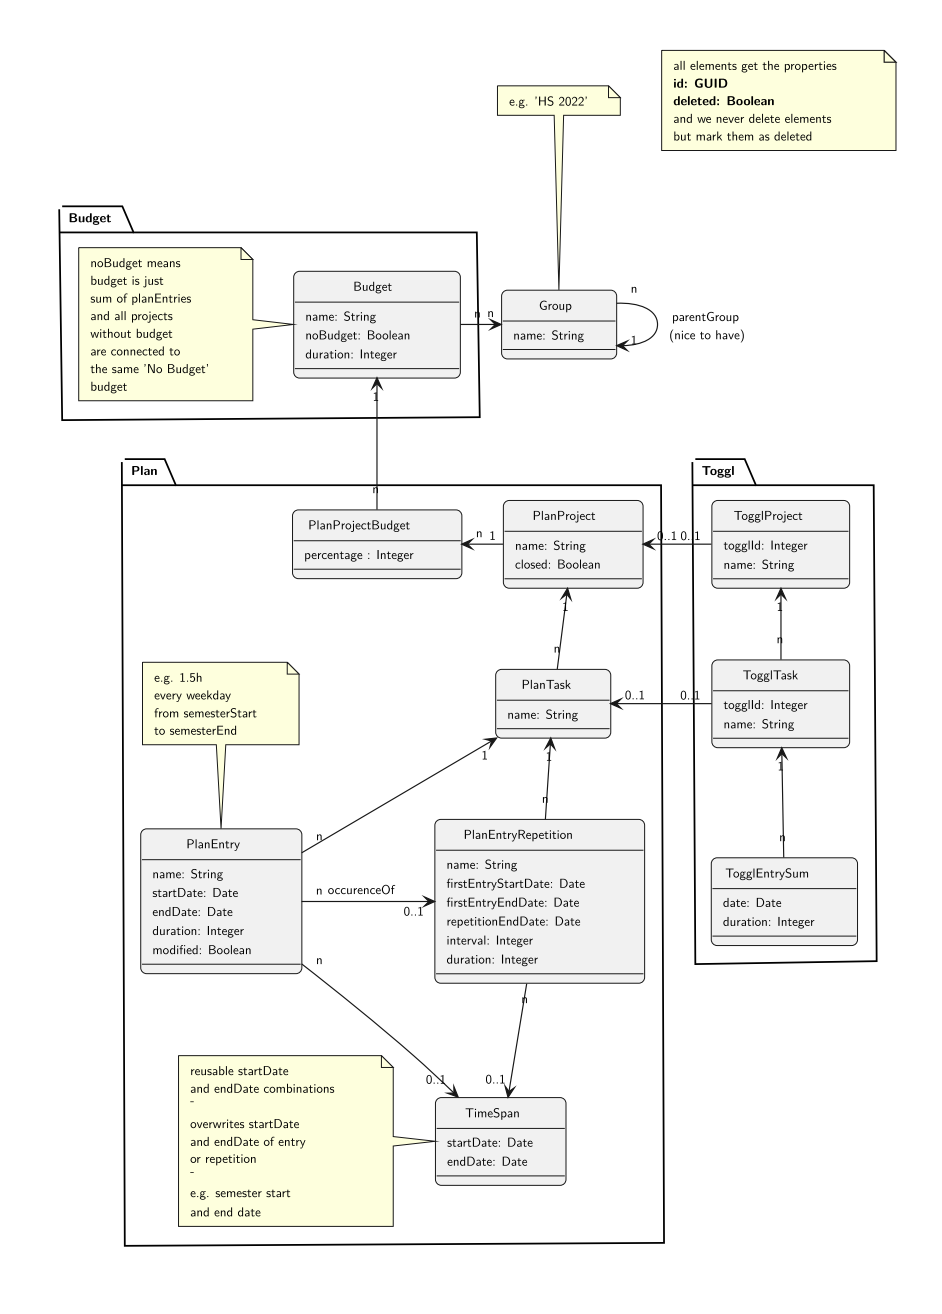
\includegraphics[width=1.0\columnwidth]{classdiagram_prototype}
	\caption{Class Diagram of the bachelor thesis prototype}
	\label{figure3}
\end{figure}

\subsection{Budget and Group}
Budgets are optional features of the ATP. They are used if a task does not have an equal distribution. For instance, the budgets allow a lecturer to allocate more time for preparing and marking of exam papers. The budgets can be divided into groups like semester or year.

\section{GitHub} \label{GitHub}
GitHub \cite{github_url} is an online service which provides Git \cite{git_url} based version control for software projects.
\subsection{Version control} \label{Version control}
Version control is used to see what was changed when and by whom. It can also be used to roll back to an older state if needed. In GitHub a feature branch is created to implement a certain feature, and afterwards when finished such a branch will be integrated into the main branch via a pull request. This pull request allows the other members of the team to request changes before the branch is merged into the main branch. This process also enables members of a team to work independently without the problem of accidentally interfering with an other team member's work.
\subsection{GitHub Actions} \label{GitHub Actions}
GitHub Actions is a (CI/CD) platform \cite{github_actions_url}. It allows for build and test automation as well as maintaining a deployment pipeline. Furthermore, workflows to automatically test and build the software on every pull request can be created. This feature helps to prevent the accidental inclusion of broken features or features which isolated work as intended but would cause other parts of the software to crash when integrated into it.
\subsection{GitHub Issues} \label{GitHub Issues}
Issues are often related to features and the corresponding feature branches. They provide the possibility to break down a milestone into manageable tasks which can then be assigned to the members of the team to work on. Thus, tasks and their assigned members can be monitored and identified. 

\section{JSON}
JSON (JavaScript Object Notation) \cite{json_url} is a data-interchange format. JSON is easily readable by humans and machines alike. It is also easy to write/generate a JSON file. Furthermore, it is language independent.\newline
JSON consists of two structures:
\begin{itemize}
	\item A collection of unordered name/value pairs. They are enclosed in curly brackets. A pair is seperated by a colon and after each name/value pair, a comma follows to separate them from the next pair.
	\item An ordered list of variables. Such a list starts with a left and ends with a right square bracket.
\end{itemize}
These two structures can be combined in a JSON file to get something akin to the JSON file shown in picture \ref{figure4}

\begin{figure}[H]
	\centering
	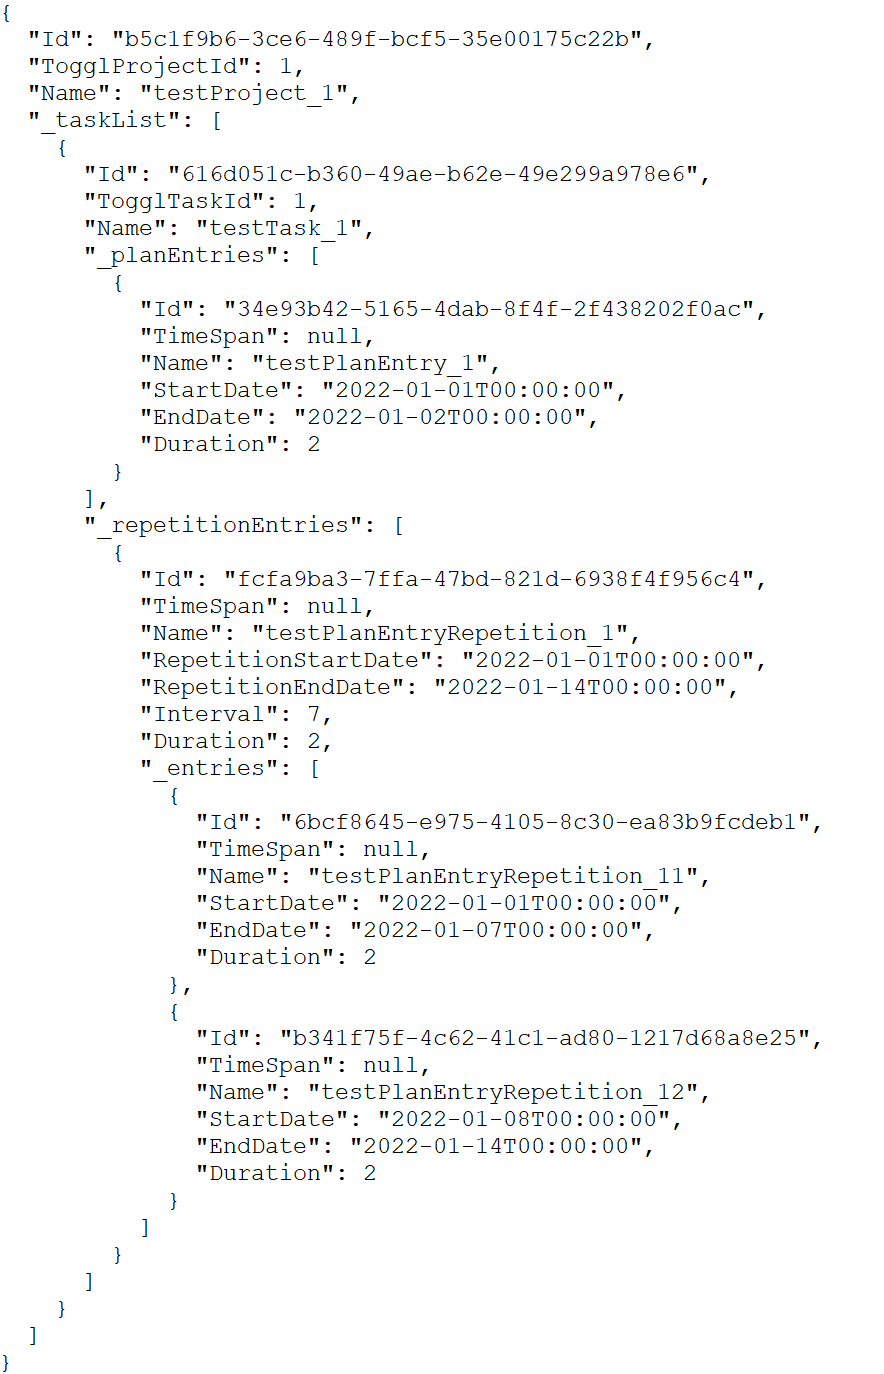
\includegraphics[width=0.7\columnwidth]{JSONExample}
	\caption{Example of a JSON file}
	\label{figure4}
\end{figure}

\section{Local Storage} \label{Local Storage}
Local Storage is a mechanism provided by the Web Storage API by which browsers can store data as key/value pairs without having to use cookies. Data stored in Local Storage persists when the browser is closed and reopened and only is deleted on cache clearing \cite{web-storage-api-url}. Moreover, the data is scoped to the browser window, which means that multiple tabs within the same browser window share the data \cite{blazor-state-management-url}. The maximum amount of data which can be stored in Local Storage is 5 MB. To access Local Storage from within a Blazor application, there is an open-source library available, which is called LocalStorage and provided by Blazored \cite{local-storage-url}.

\section{C\#}
C\# is "[...] a powerful and widely used programming language that you can use to make websites, games, mobile apps, desktop apps and more with .NET. [...]" \cite{csharp-url}.

\chapter{Methods}
%%% Local Variables:
%%% mode: latex
%%% TeX-master: "../doc"
%%% coding: utf-8
%%% End:
% !TEX TS-program = pdflatexmk
% !TEX encoding = UTF-8 Unicode
% !TEX root = ../doc.tex

This section describes the approaches and methods applied in the project. These consist of the general approach, the organisation methodology chosen, the use of Git version control and the project schedule set up at the beginning of the project.

\section{Realization of project}
The following subsections describe the realization of the project in detail.

\subsection{Proof that approach of bachelor thesis is applicable}
The first step as to realisation of this project was to prove whether the approach given by the bachelor thesis on which the project is founded is applicable. Since neither one of us has ever worked with Blazor or the related technologies used in the bachelor thesis, the consideration of the software prototype was of particular importance. Both the prototype (see chapter tbd) and the concept of mapping Toggl Track data to ATP data (see chapter tbd) have been investigated in detail. This was done using the documentation of the bachelor thesis, the software code of the prototype and the Blazor online documentation. Thus a fundamental understanding of the approach has been gained. Moreover, our .NET teacher, Mr. Rege, has agreed to provide technological support for Blazor and related technologies. In the light of all this, the approach has been considered applicable and therefore served as basis for the realisation of this project.

\subsection{Implementation of mapping concept}
To be able to actually handle data in the application, the mapping concept designed in the bachelor thesis (see chapter \ref{Mapping concept}) had to be implemented. The implementation generally follows the mapping concept apart from a few class attributes which were deleted since they were not considered to be needed.

\subsection{Graphical overview of difference between planning and tracking}
Since the comparison between planned and tracked time should be displayed graphically, there had to be a possibility to display data using charts. The approach suggested in the bachelor thesis was to use the JavaScript library Charts.js and call it directly out of the application. However, this was not considered to be the best way to display charts since JavaScript code had to be added manually and called using code injection. Therefore, we decided to dedicate some time to investigate more elegant alternatives. The following packages offer functionality to create charts in Blazor without having to write JavaScript code:
\begin{itemize}
	\item Blazorise \cite{blazorise-url} - a multi-component library providing charts display functionality via an extension
	\item ChartsJs.Blazor \cite{chartsjs.blazor-url} - an open-source interface to the Charts.js JavaScript library
	\item Plotly.Blazor \cite{plotly-url} - an open-source charts display library available in multiple languages
	\item Radzen \cite{radzen-url} - a multi-component library
\end{itemize}
All four packages were tested by trying to include a sample chart into the application. Apart from ChartsJs.Blazor, which happened to have some installation issues, all packages could easily be installed and integrated. The following pictures show sample charts generated by the different packages being displayed in the ATP.

\begin{figure}[H]
	\centering
	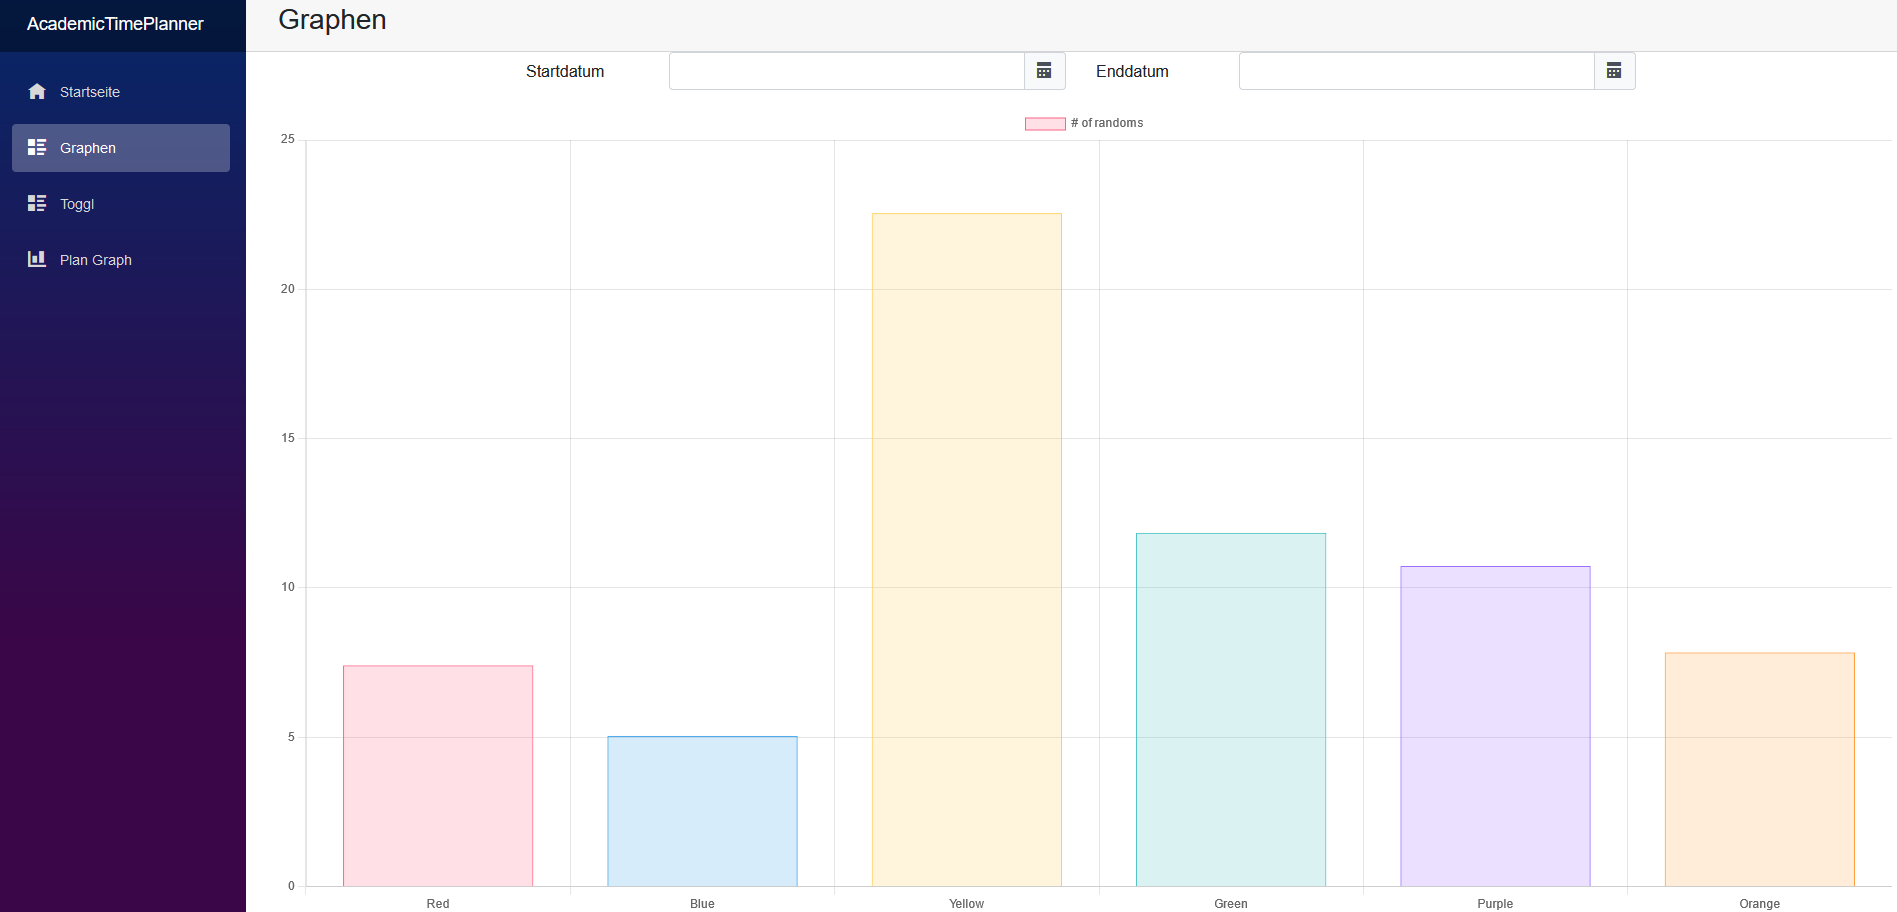
\includegraphics[width=1.0\columnwidth]{blazorise-charts}
	\caption{Blazorise sample charts on the ATP charts page}
	\label{figure5}
\end{figure}

\begin{figure}[H]
	\centering
	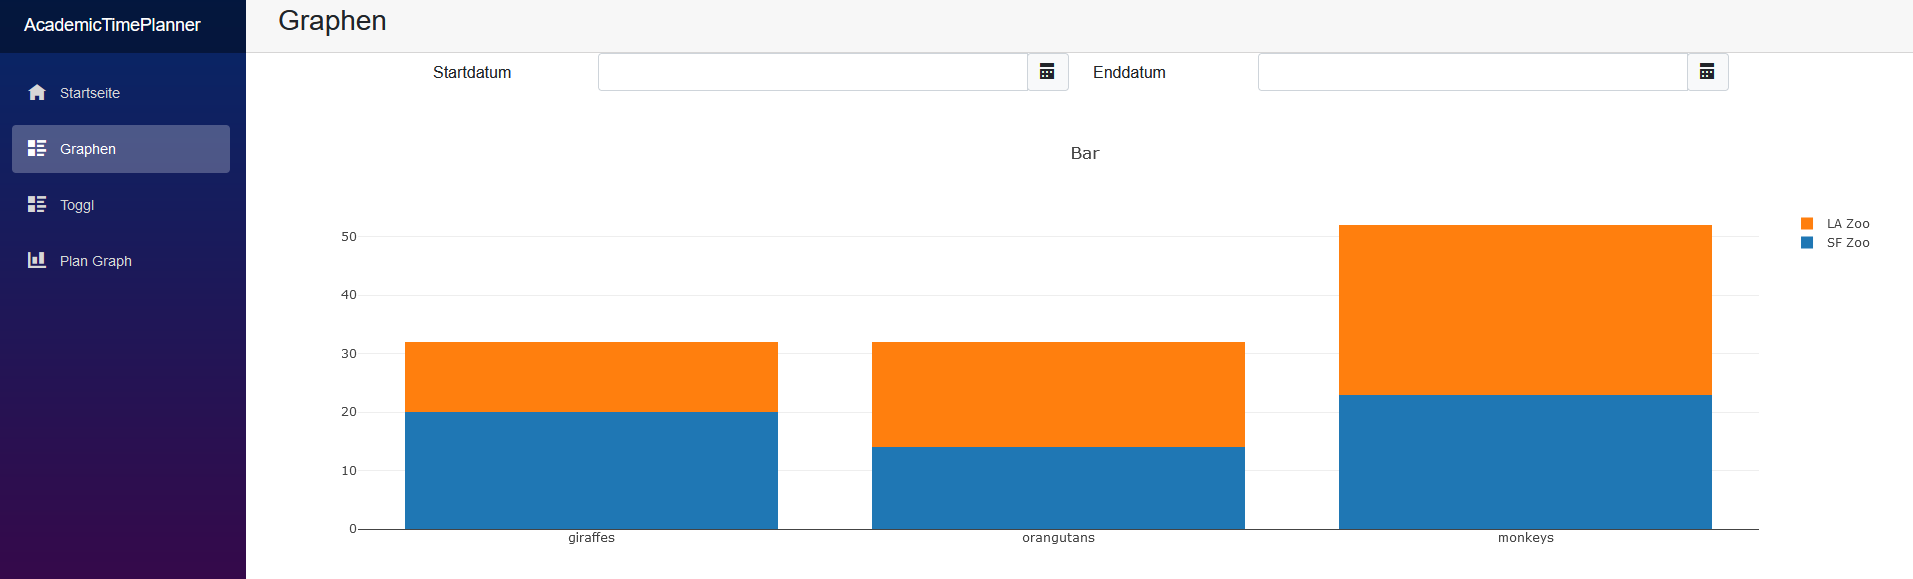
\includegraphics[width=1.0\columnwidth]{plotly-charts}
	\caption{Plotly.Blazor sample charts on the ATP charts page}
	\label{figure6}
\end{figure}

\begin{figure}[H]
	\centering
	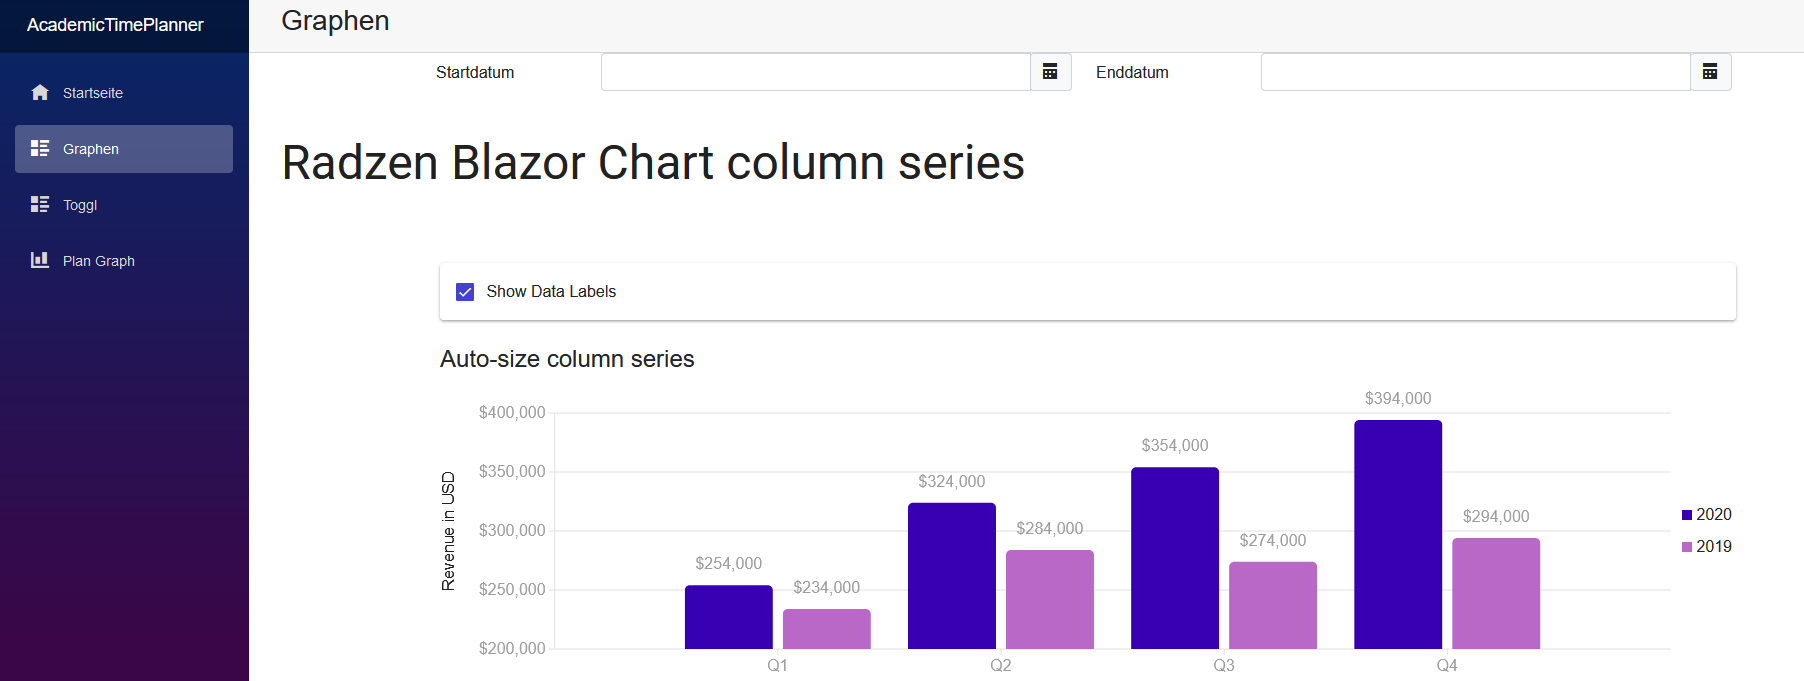
\includegraphics[width=1.0\columnwidth]{radzen-charts}
	\caption{Radzen sample charts on the ATP charts page}
	\label{figure7}
\end{figure}

For the realisation of the charts display, Plotly.Blazor was deemed to be the most suitable package for this application, since it focuses on exactly that functionality and is easier to use, compared to the other packages named above. The result of the implementation is described in more detail in chapter \ref{Graphical overview}

\subsection{Test projects}
To correctly simulate a working environment, test projects were created. To use a Toggl project in the application without actually having to fetch data from the Toggl API, a helper class providing a simulated Toggl project was created. A JSON file containing simulated planned data allowed for loading and using a plan project in the application. The combination of these two projects allowed the whole application to run without the need for real data while still displaying reasonable values for the user.

\section{Organization methodology}
For this project a reduced and modified version of SCRUM \cite{scrum_url} was chosen. The modifications include reducing the daily SCRUM meetings to two to three meetings a week, as we did not work on the project full time. One of these meetings was also attended by our project advisor Mr. Feisthammel. This meeting was usually held on Tuesday morning. There, a short progress report as well as the next weekly goals were discussed. Milestones as described in chapter \ref{Time management} have been defined. They roughly correspond with the two-week sprint plan. An additional reduction is the absence of a sprint review as we do something similar in the weekly meetings described above. The point system as well as the burn down chart were also dropped.

\section{Git}
For appropriate software code management, the Git version control system and the online service GitHub (see chapter \ref{Version control}) have been used. The software code was stored in a GitHub repository named "academic-time-planner". The main branch always represented the current state of the software, containing all tested and approved features. New features were implemented via feature branches named according to the pattern "feature/name-of-member/feature-description". The software tests were executed automatically via GitHub Actions (see chapter \ref{GitHub Actions}) on every push to a feature branch. The result of the automated tests were taken into account in the feature pull requests. The documentation was kept in the same repository and was treated like the software code in the sense that additions and changes had to be reviewed and approved via pull requests, as was the software code. Documentation branches were named after the "documentation/name-of-member/section-description". Tasks were managed via GitHub issues (see chapter \ref{GitHub Issues}).

\section{Time management} \label{Time management}
Four milestones were proposed at the beginning of the project. They were taken from the project outline and include three programming milestones and one documentation milestone. The first one was the implementation of the overview of difference between plan and tracking, followed by the application status display. The final programming milestone was composed of the import and export as well as the creation of plan projects. After this the documentation had to be finalized. These milestones were meant as a guideline to see if the progress was adequate or if we had to rethink our approach. Those milestones were created and managed in GitHub (see chapter \ref{GitHub}). 





\chapter{Results}
%%% Local Variables:
%%% mode: latex
%%% TeX-master: "../doc"
%%% coding: utf-8
%%% End:
% !TEX TS-program = pdflatexmk
% !TEX encoding = UTF-8 Unicode
% !TEX root = ../doc.tex

This chapter shows the results achieved during realization of the project.

\section{Architectural overview} \label{Architecture}
In this section the software architecture of the ATP is shown as realized.

\subsection{Packages}
The following packages form the architecture of the ATP:
\begin{itemize}
	\item Pages: pages of the UI and their controller code
	\item Shared: common parts of the pages and their controller code
	\item UIModels: helper classes needed by the pages to map entry form elements to
	\item Services: classes providing functionality to fetch data from Toggl or Local Storage, being provided to other classes via dependency injection
	\item Store: classes managed by Fluxor to handle user inputs from and provide outputs to the pages, using services for data fetching
	\item DataManagement: business logic managing application data, made persistent by being saved in Local Storage
	\item Data: consists of ApplicationData (classes modelling planning and Toggl data), DisplayData (planning and Toggl data as used by the UI) and MetaData (additional data used by the ATP, e.g. Toggl credentials).
	\item JSONHandling: helper classes for JSON data handling (used in tests and by Local Storage)
\end{itemize}
The Program.cs file is the entry point of the system where the application is set up and run. \_Imports.razor, App.razor and wwwroot contain global application settings. The packages and their relations are shown in figure \ref{architecture_overview}. Packages containing UI functionality are marked blue, packages managed by external frameworks are marked violet, services are marked orange, business logic is marked green, and data packages are marked red.
\begin{figure}[H]
	\centering
	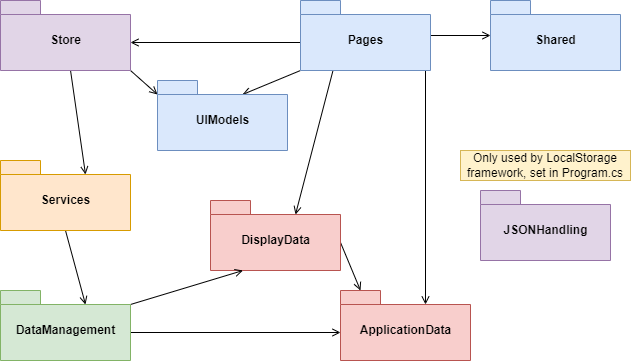
\includegraphics[scale=0.5]{Architecture_overview}
	\caption{Architectural overview}
	\label{architecture_overview}
\end{figure}

\subsection{Mapping concept} \label{Mapping_result}
Upon closer inspection it became apparent that only four of the plan classes and two of the Toggl classes were needed. The Toggl tasks are currently only a dictionary inside the TogglProject class and not a class in their own right. The Budget classes were implemented differently as a feature of the plan projects. Each plan project keeps the Toggl projects linked to it with their share of time. The share of time for a Toggl project is calculated as follows:
\begin{equation*}
	Share \, of \, time = \frac{Total \, time \, of \, plan \, project}{Sum \, of \, total \, times \, of \, all \, plan \, projects \, linked \, to \, Toggl \, project}
\end{equation*}
With all these modifications the class diagram of the mapping concept was slimmed down as seen in figure \ref{classdiagram_prototype_current}.
\begin{figure}[H]
	\centering
	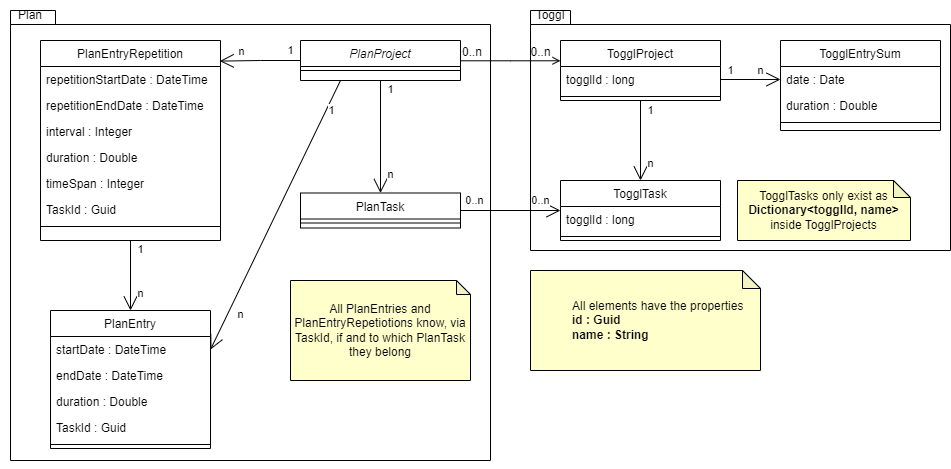
\includegraphics[width=1.0\columnwidth]{classdiagram_prototype_current}
	\caption{Class diagram of the new mapping concept}
	\label{classdiagram_prototype_current}
\end{figure}

\section{Application data persistence with LocalStorage}
The approach described in chapter \ref{Local Storage} was applied to store application data (plan project data, data fetched from Toggl etc.). The data is held by a data manager object which is stored in LocalStorage and can be loaded from there using the interface provided by the LocalStorage library.

\section{Overview PlanProject vs TogglProject} \label{Graphical overview}
Three different charts are displayed in the charts tab to display the difference between the plan projects and the corresponding Toggl projects.
\begin{itemize}
	\item Total overview
	\item Projects overview
	\item Project time range overview
\end{itemize}
The different charts are explained in more detail in the following subsections.

\subsection{Total Overview}
This bar chart shows the overall sum of the time planned for all plan projects compared to the total tracked time of their associated Toggl projects. Additionally, a prediction of how much time will be needed according to the future plan entries is displayed. An example for two projects is shown in figure \ref{totalOverview}.
\begin{figure}[H]
	\centering
	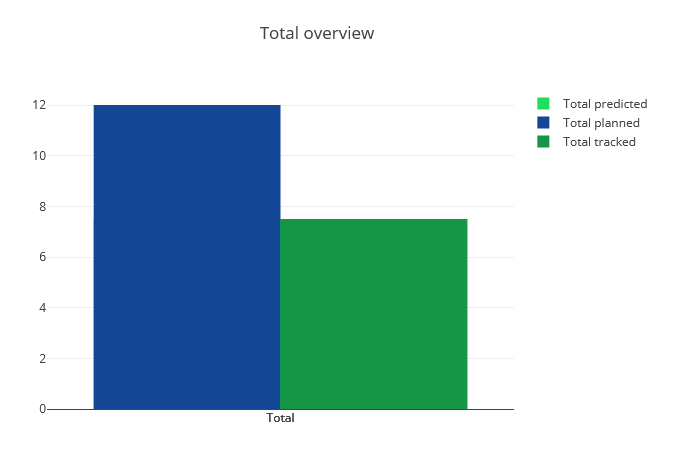
\includegraphics[width=1.0\columnwidth]{TotalOverview}
	\caption{Total overview for all projects}
	\label{totalOverview}
\end{figure}
If all projects have been completed already meaning there are no future plan entries for any project then no prediction will be displayed. An example for one project is shown in figure \ref{totalOverviewFinished}.
\begin{figure}[H]
	\centering
	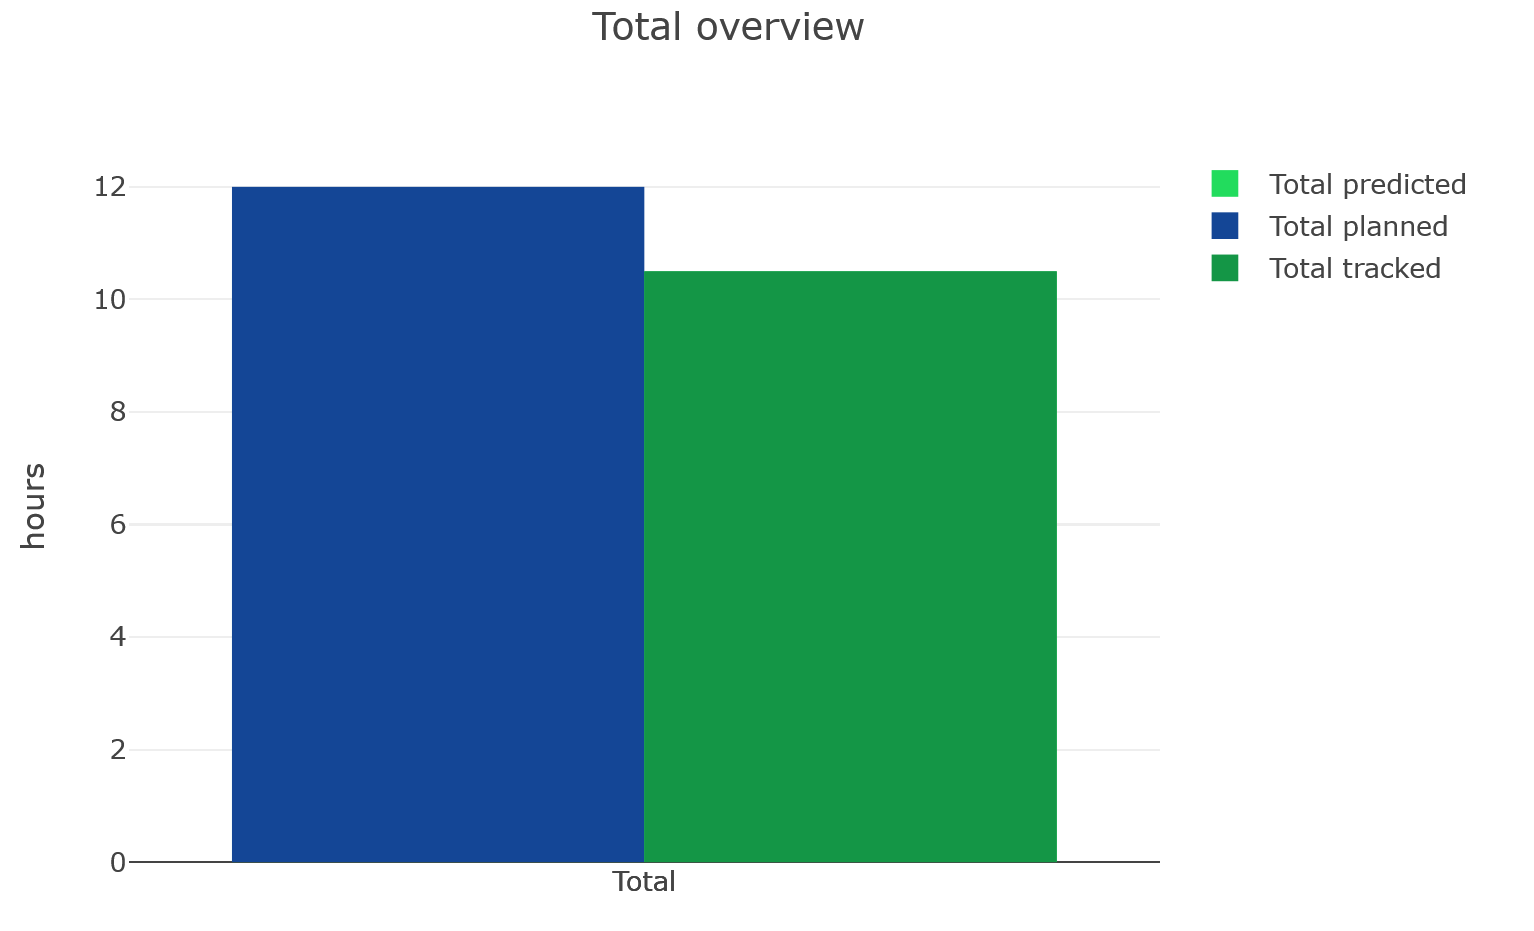
\includegraphics[width=1.0\columnwidth]{TotalOverview_FinishedProject}
	\caption{Total overview for one finished project}
	\label{totalOverviewFinished}
\end{figure}

\subsection{Projects Overview}
This bar chart is similar to the total overview but the single projects are displayed separately. Another minor difference is that the prognosis is added to both the tracked time and the planned time creating a prediction for both. The prediction is calculated by subtracting the time planned until today from the total planned time. Time planned until today is calculated by summing up all entries with start dates in the past. Currently running entries are added by percentage (e.g. in a week long entry beginning at Monday, Friday would be approximately 71.43\%). An example for two projects is shown in figure \ref{projectOverview}.
\begin{figure}[H]
	\centering
	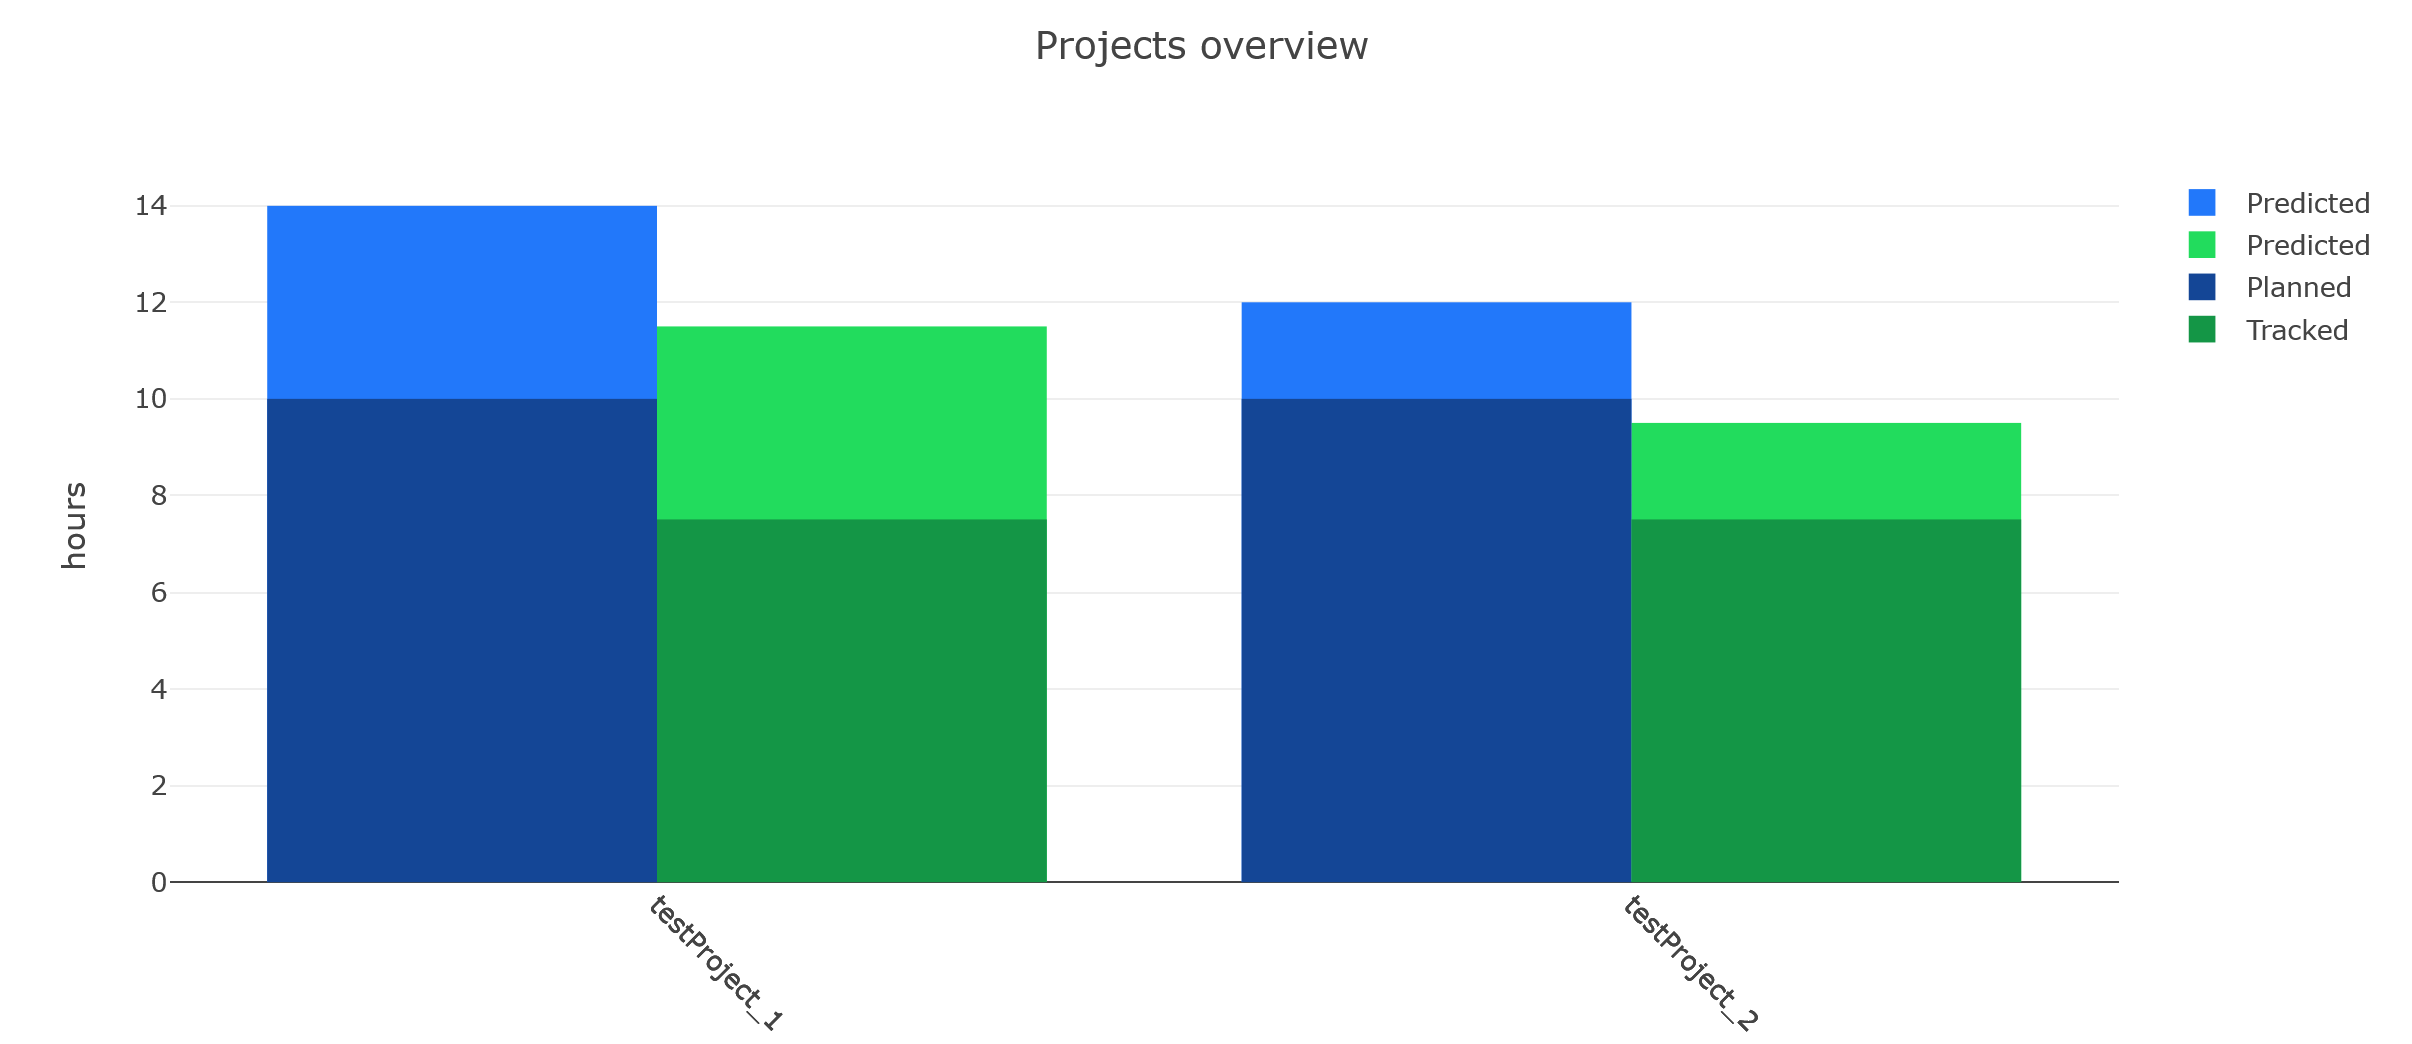
\includegraphics[width=1.0\columnwidth]{ProjectOverview}
	\caption{Project overview for two projects}
	\label{projectOverview}
\end{figure}
If a project has been completed already meaning there are no future plan entries for it then no prediction will be displayed for that project. An example for one project is shown in figure \ref{projectOverviewFinished}.
\begin{figure}[H]
	\centering
	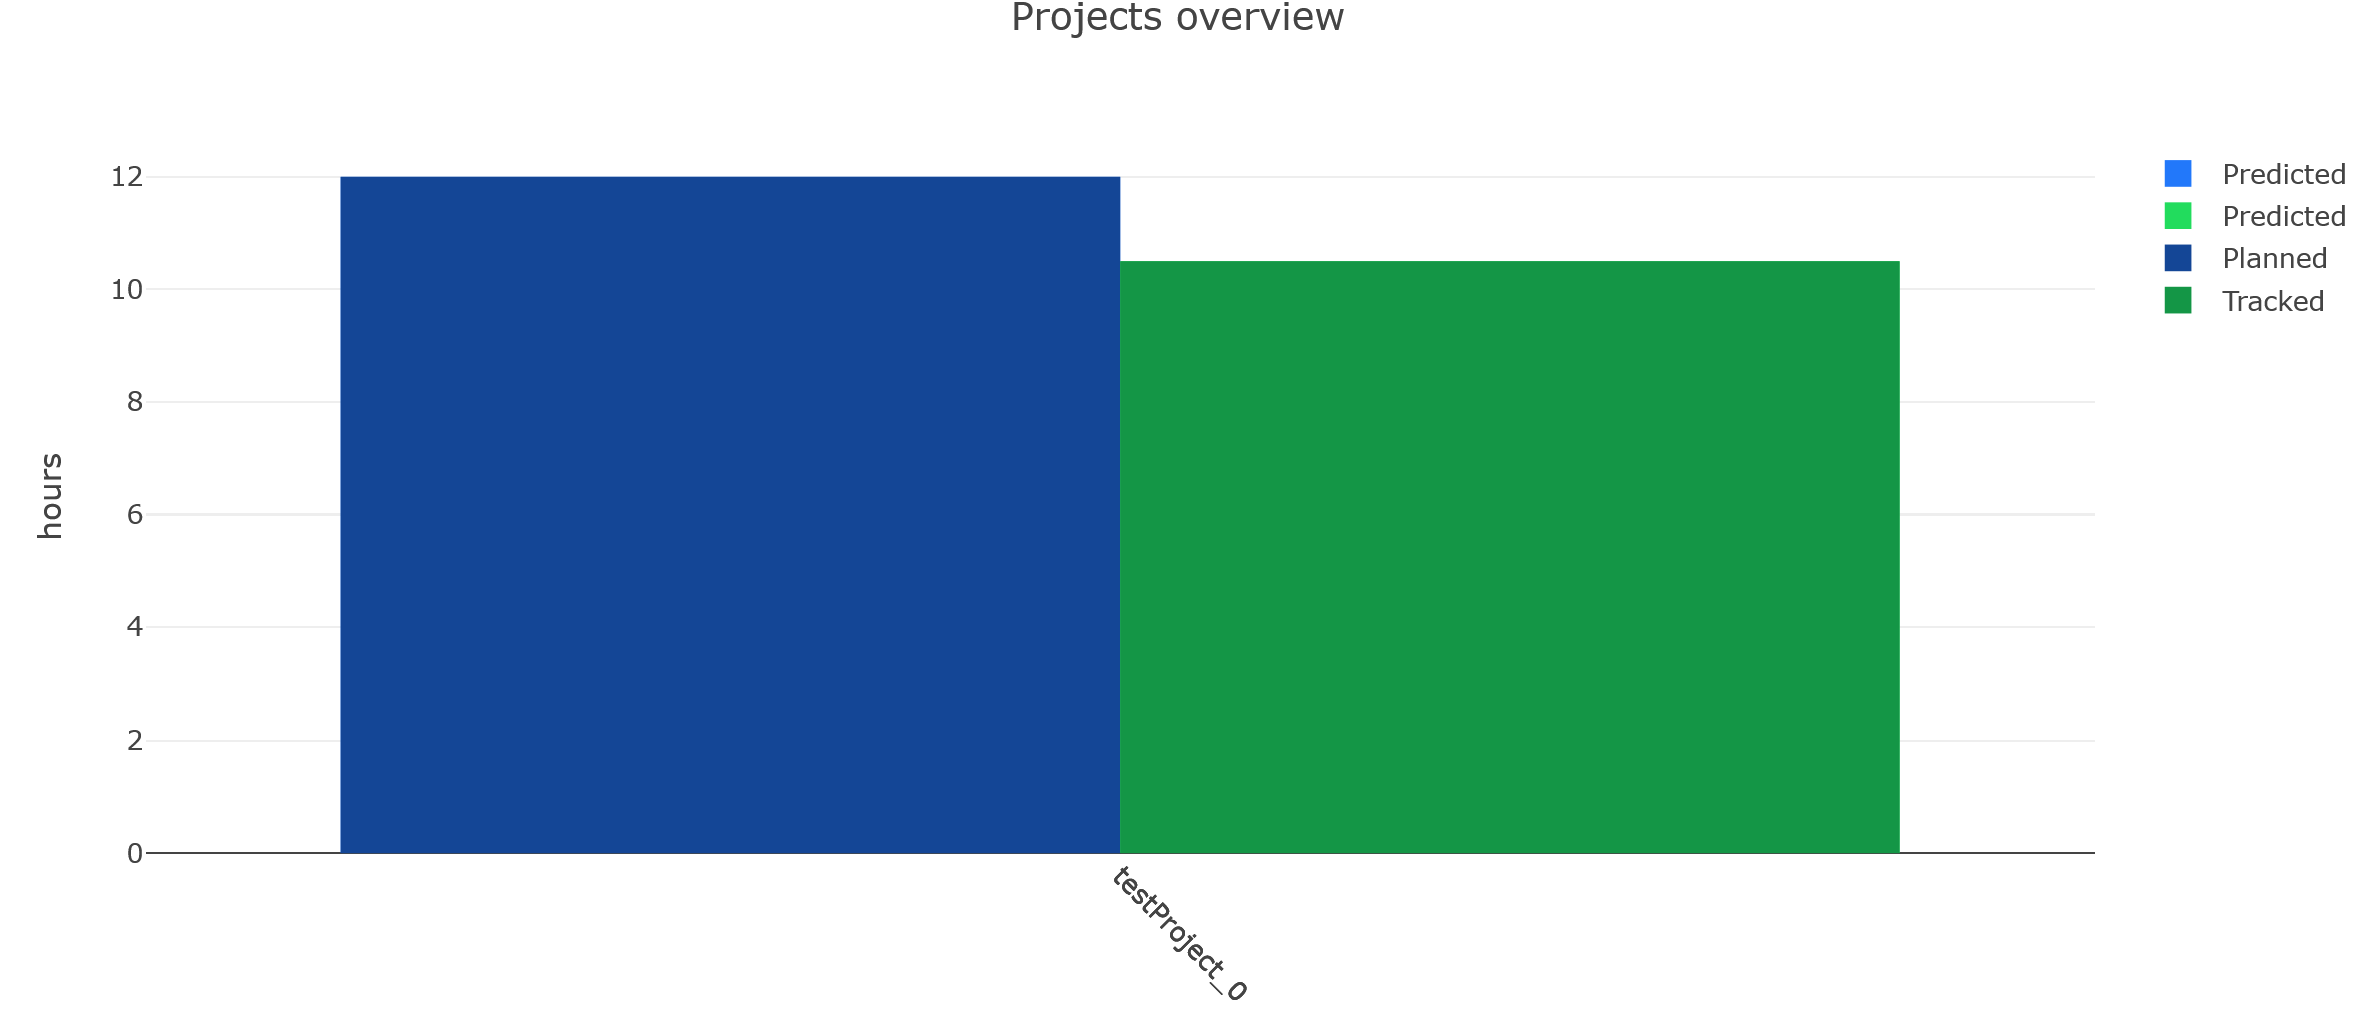
\includegraphics[width=1.0\columnwidth]{ProjectOverview_FinishedProject}
	\caption{Project overview for one finished project}
	\label{projectOverviewFinished}
\end{figure}

\subsection{Project time range overview}
An applicable time range has to be chosen to display the chart. On hitting the "Set filter" button the time range is set and a line chart is drawn for every project, showing the development of planned time and tracked time during the selected time range. The "Reset filter" button deletes the charts and reopens the filter options. This chart allows to see how the time amounts displayed in the other charts have been achieved and thus enables a user to estimate the quality of their planning. An example for one project is shown in figure \ref{timeOverview}.
\begin{figure}[H]
	\centering
	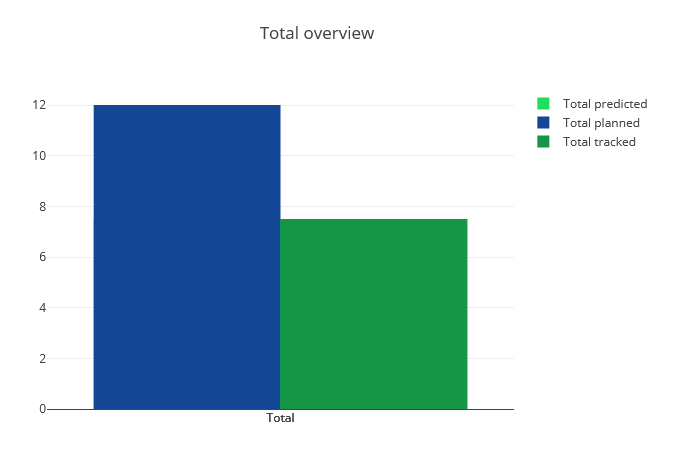
\includegraphics[width=1.0\columnwidth]{TimeOverview}
	\caption{Time overview for one project}
	\label{timeOverview}
\end{figure}

\section{Application status display and synchronization} \label{Status display}
A Blazor page for synchronization with Toggl had already been added in the original prototype. The modal entry mask was replaced by Blazor input components as described in chapter \ref{JS replacement} (see figure \ref{Toggl page initial}). When the "Save Toggl settings" button is clicked the credentials entered in the text fields are saved using Local Storage (see chapter \ref{Local Storage}) and a first synchronization request is sent to Toggl. If one or both fields are left empty, appropriate error messages are displayed (see figure \ref{Toggl page validation}). After successful synchronization, the entry fields and the save button are replaced by a "Synchronize" button in order to allow users to re-synchronize the ATP with Toggl at any time and not just on entering the Toggl credentials. A label next to the button indicates the time of the last synchronization. An overview of the loaded data and their associations with the ATP planning data is displayed below the button (see figure \ref{Toggl associated}). If a Toggl project has no associations yet it is indicated in the load overview (see figure \ref{Toggl loaded}). Entries which do not belong to a Toggl project are displayed as belonging to "Entries without project" (see figure \ref{Toggl no project}). Internally, these entries are saved in a project having this name. Toggl projects which have been deleted in Toggl, but are still present in the ATP, are marked as deleted (see figure \ref{Toggl deleted}). They will be present in the ATP until Local Storage is cleared (e.g., when the browser cache is cleared).

\begin{figure}[H]
	\centering
	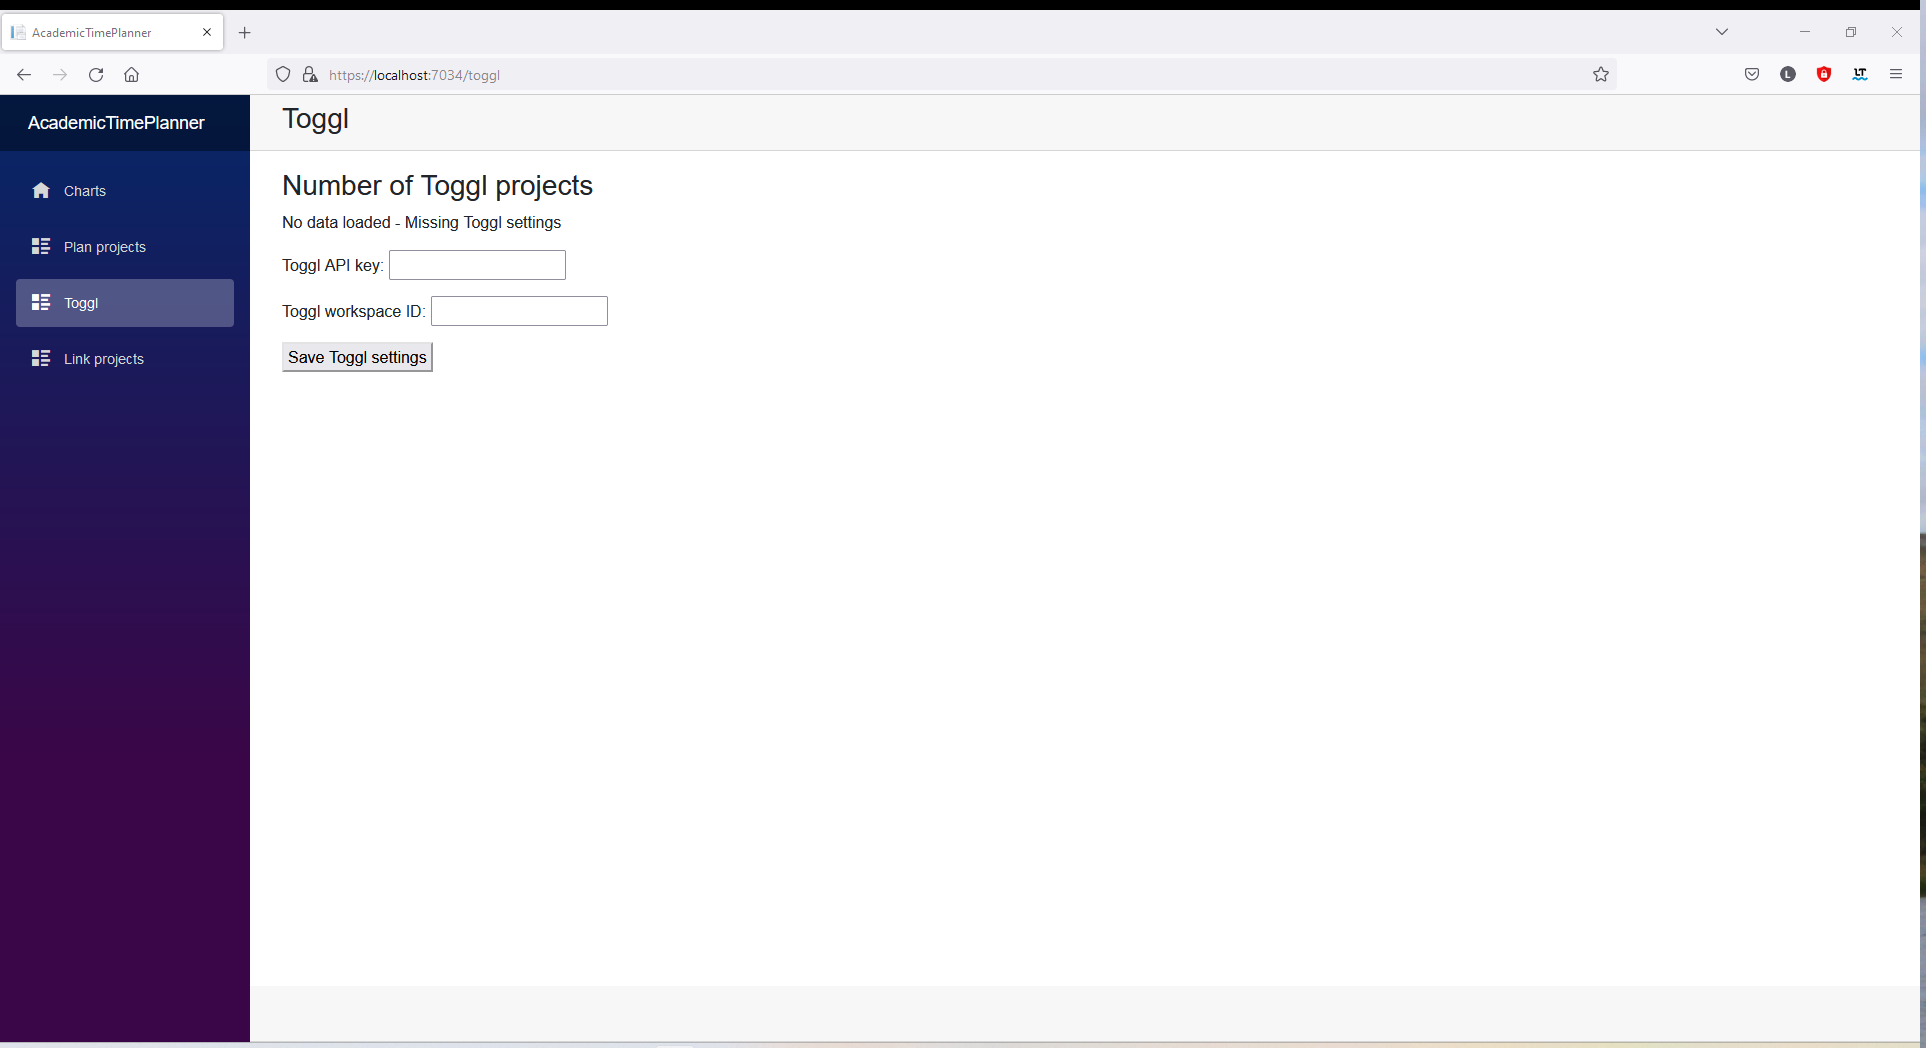
\includegraphics[scale=0.75]{Toggl_init}
	\caption{Toggl page with no Toggl projects loaded prior to synchronization}
	\label{Toggl page initial}
\end{figure}

\begin{figure}[H]
	\centering
	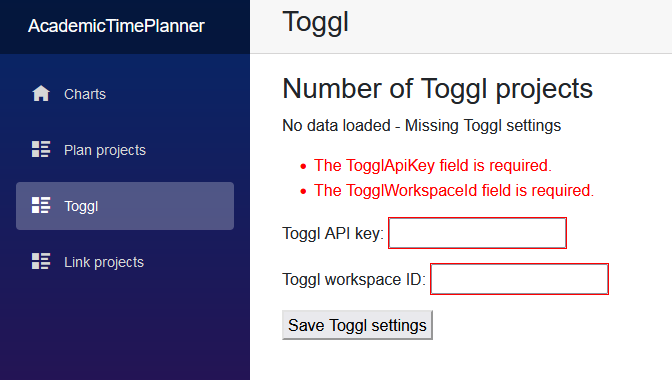
\includegraphics[scale=0.75]{Toggl_validation}
	\caption{Toggl page with empty credentials input}
	\label{Toggl page validation}
\end{figure}

\begin{figure}[H]
	\centering
	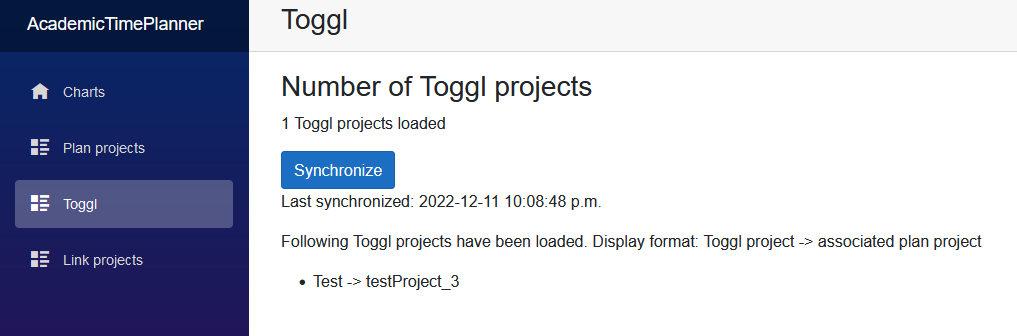
\includegraphics[scale=0.75]{Toggl_associated}
	\caption{Toggl page after loading of one Toggl project which is associated with a plan project}
	\label{Toggl associated}
\end{figure}

\begin{figure}[H]
	\centering
	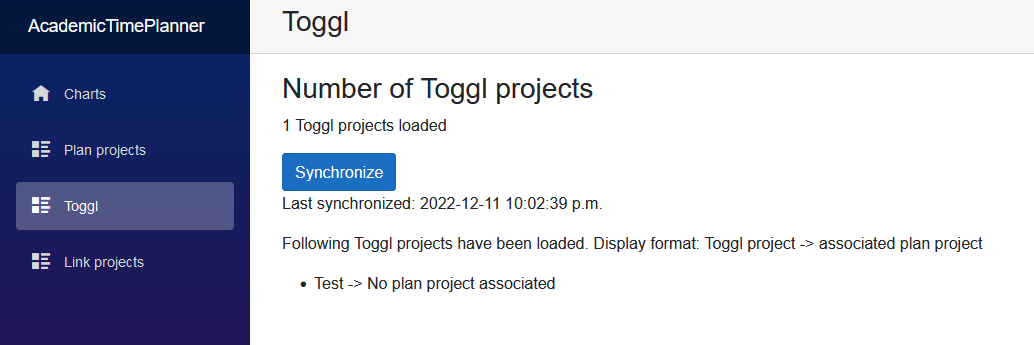
\includegraphics[scale=0.75]{Toggl_loaded}
	\caption{Toggl page after loading of one Toggl project which is not associated with any plan project}
	\label{Toggl loaded}
\end{figure}

\begin{figure}[H]
	\centering
	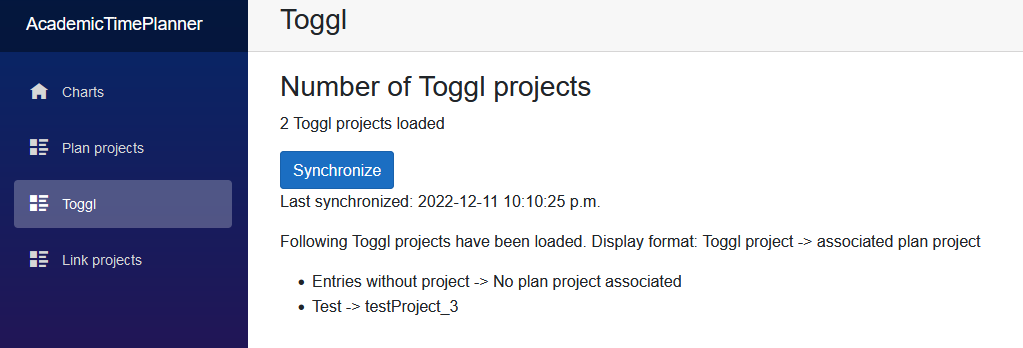
\includegraphics[scale=0.75]{Toggl_noProject}
	\caption{Toggl page after loading of a Toggl project and some entries which do not belong to a Toggl project}
	\label{Toggl no project}
\end{figure}

\begin{figure}[H]
	\centering
	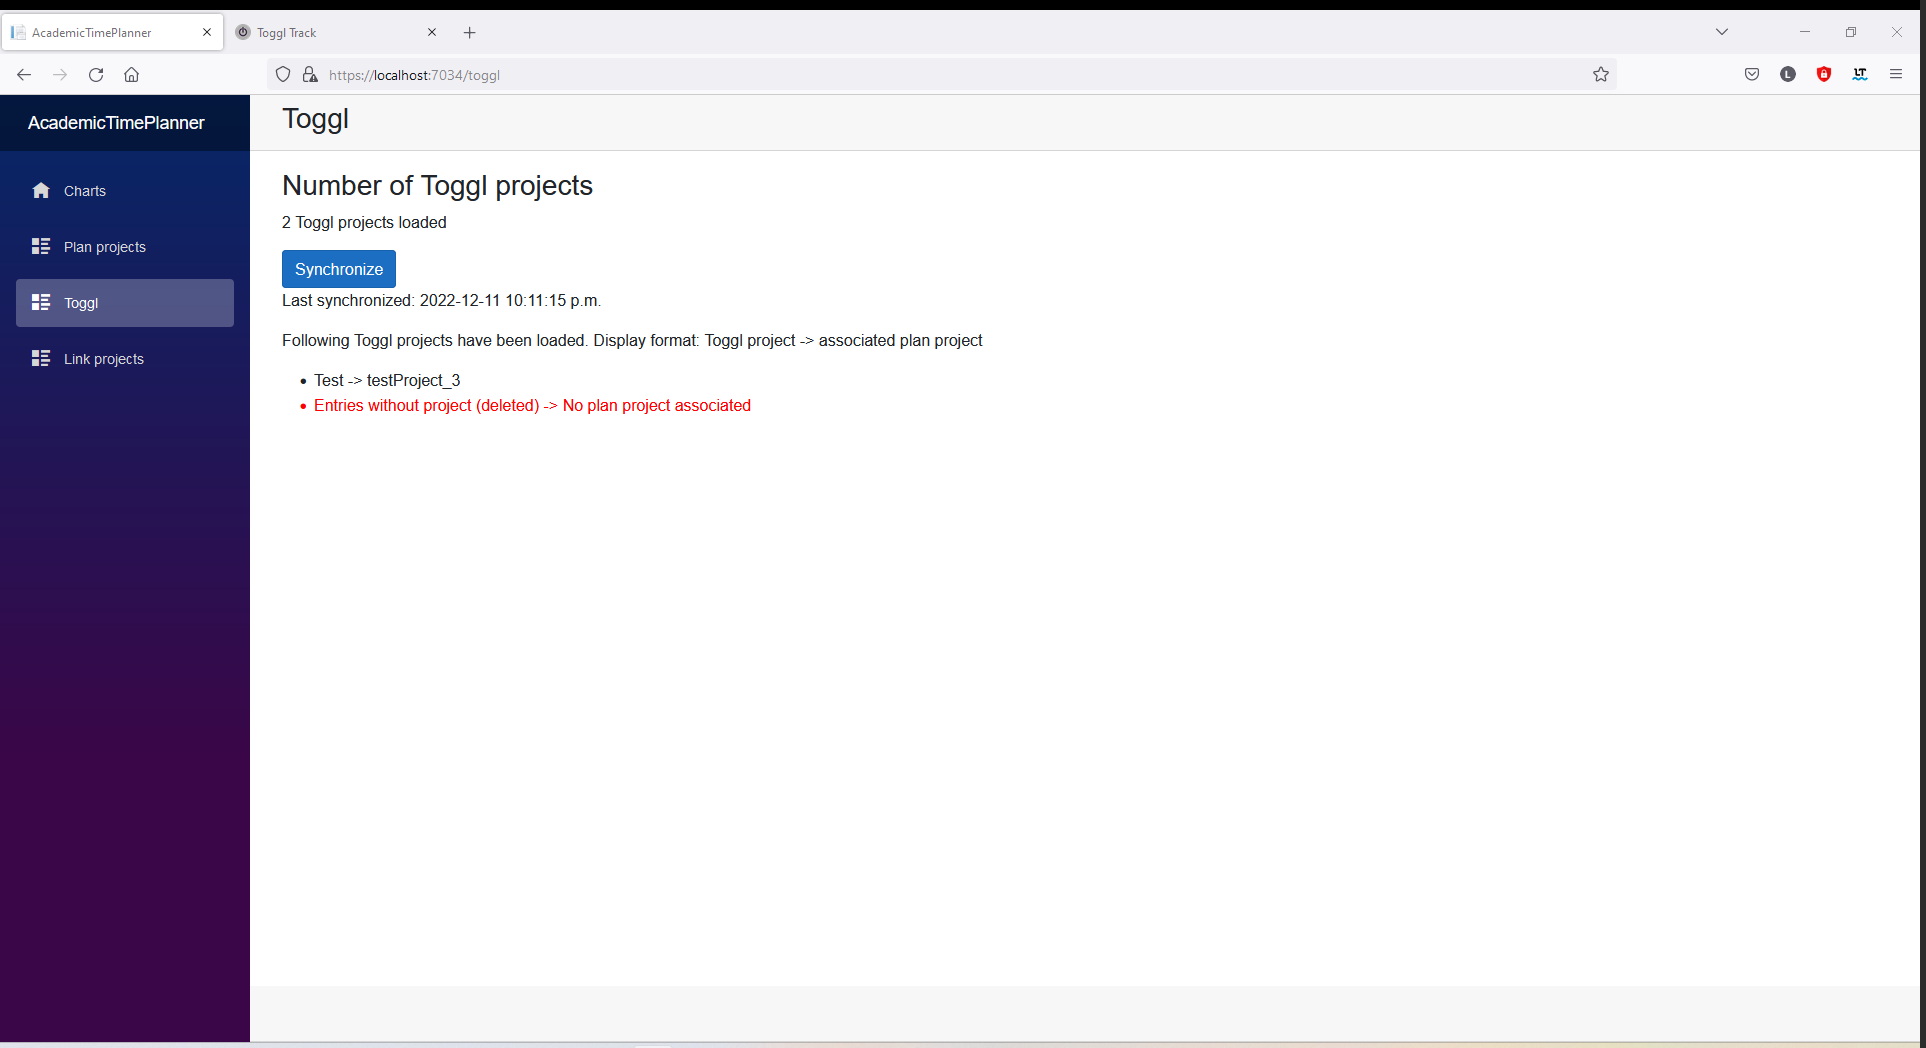
\includegraphics[scale=0.75]{Toggl_deleted}
	\caption{Toggl page after loading of one Toggl project with one deleted project}
	\label{Toggl deleted}
\end{figure}

\section{Front-end of import, export, creation and editing of plan projects}
The following subsections describe the front-end for import, export and creation of a plan project.

\subsection{Import front-end}
 The user has to click on the "Browse..." button to import a project (see figure \ref{importButton}). Doing so opens a window where the user can select the projects to be loaded (see figure \ref{importWindow}). If a project already exists in the ATP it will be overwritten with the new data otherwise the plan project is added to the ATP. All loaded plan projects are displayed in a list (see figure \ref{loadedPlanProjects}).
\begin{figure}[H]
	\centering
	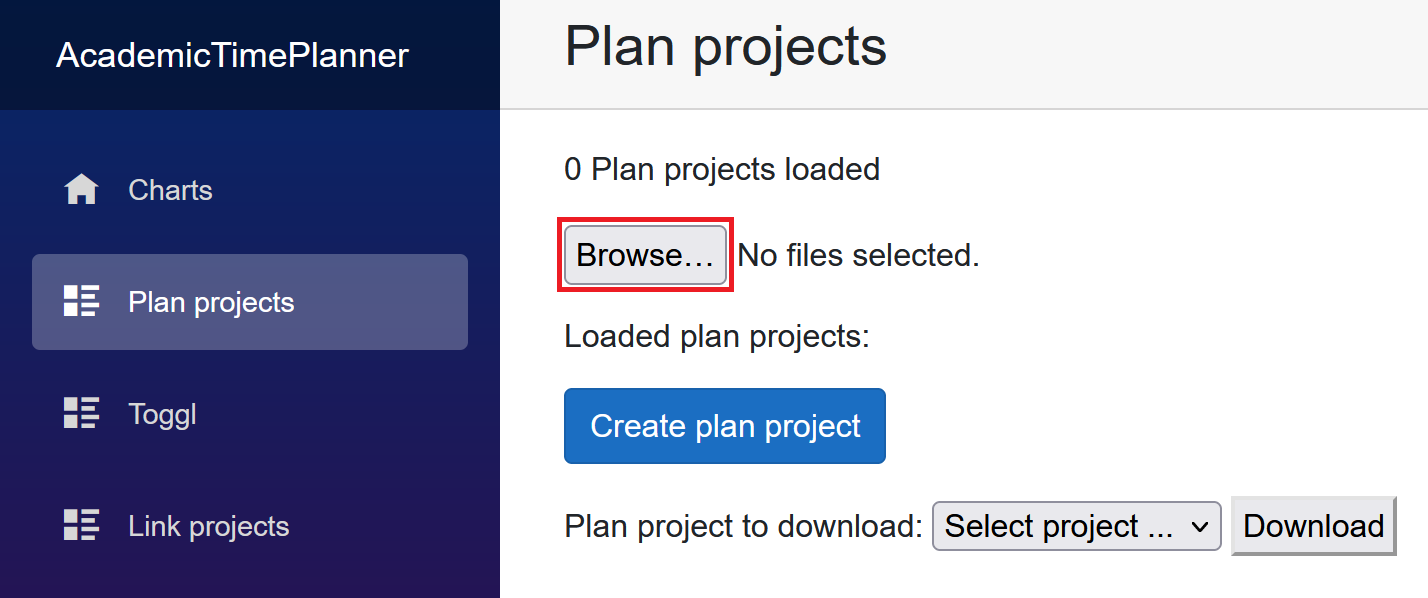
\includegraphics[scale=0.5]{ImportButton}
	\caption{Button to browse files for import}
	\label{importButton}
\end{figure}
\begin{figure}[H]
	\centering
	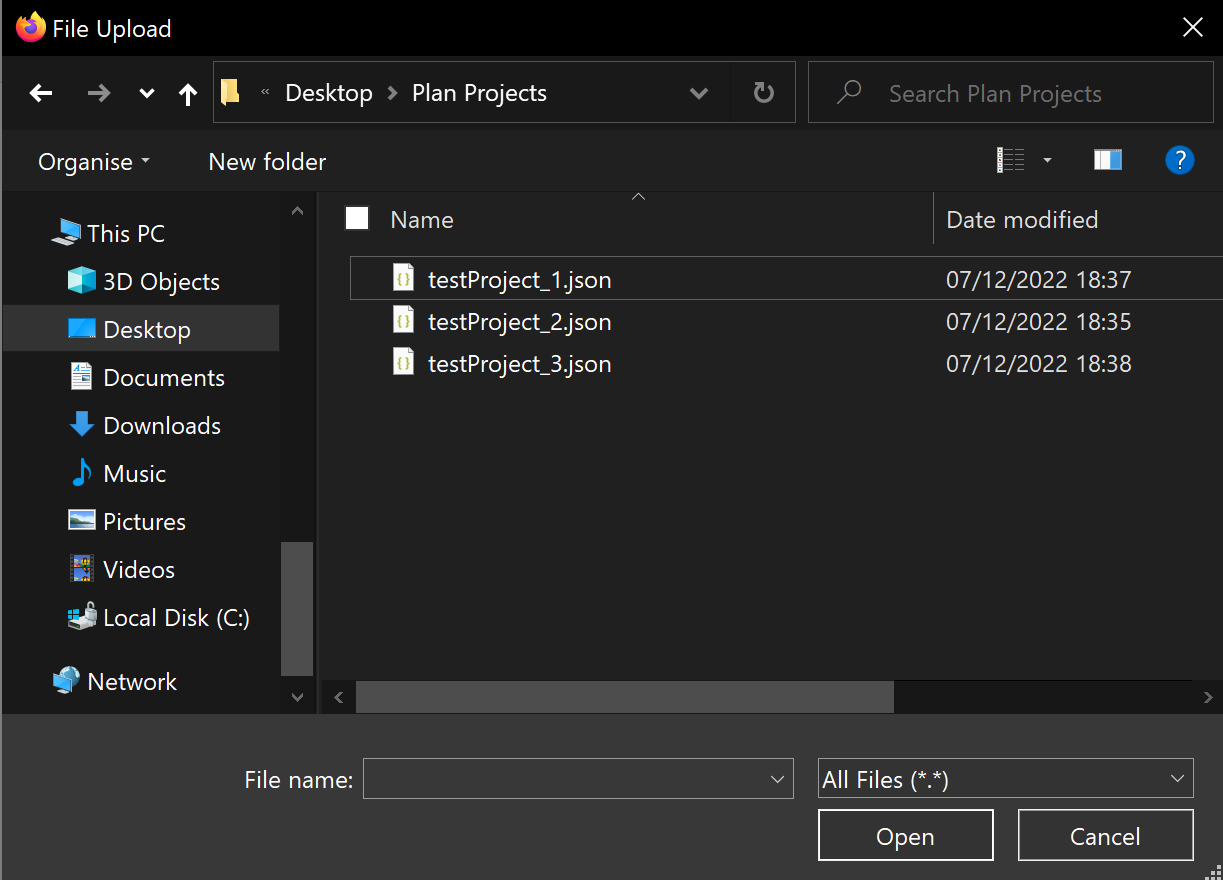
\includegraphics[width=0.6\columnwidth]{ImportProjectWindow}
	\caption{Window to select files for import}
	\label{importWindow}
\end{figure}
\begin{figure}[H]
	\centering
	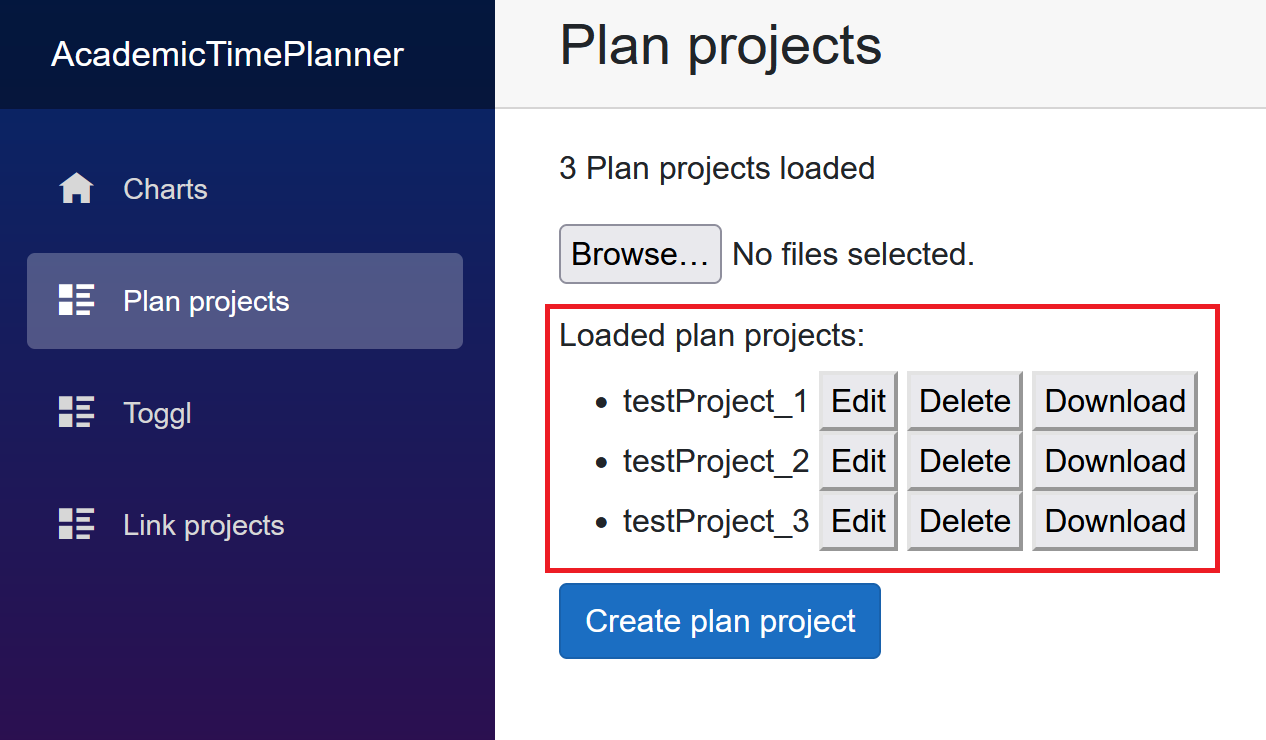
\includegraphics[scale=0.5]{LoadedPlanProjectsList}
	\caption{List of loaded plan projects}
	\label{loadedPlanProjects}
\end{figure}

\subsection{Export front-end}
The user has to click on the "Download" button next to a plan project to export it (see figure \ref{downloadButton}). This will open the browser's download options like "Save as..." or "Open with...".
\begin{figure}[H]
	\centering
	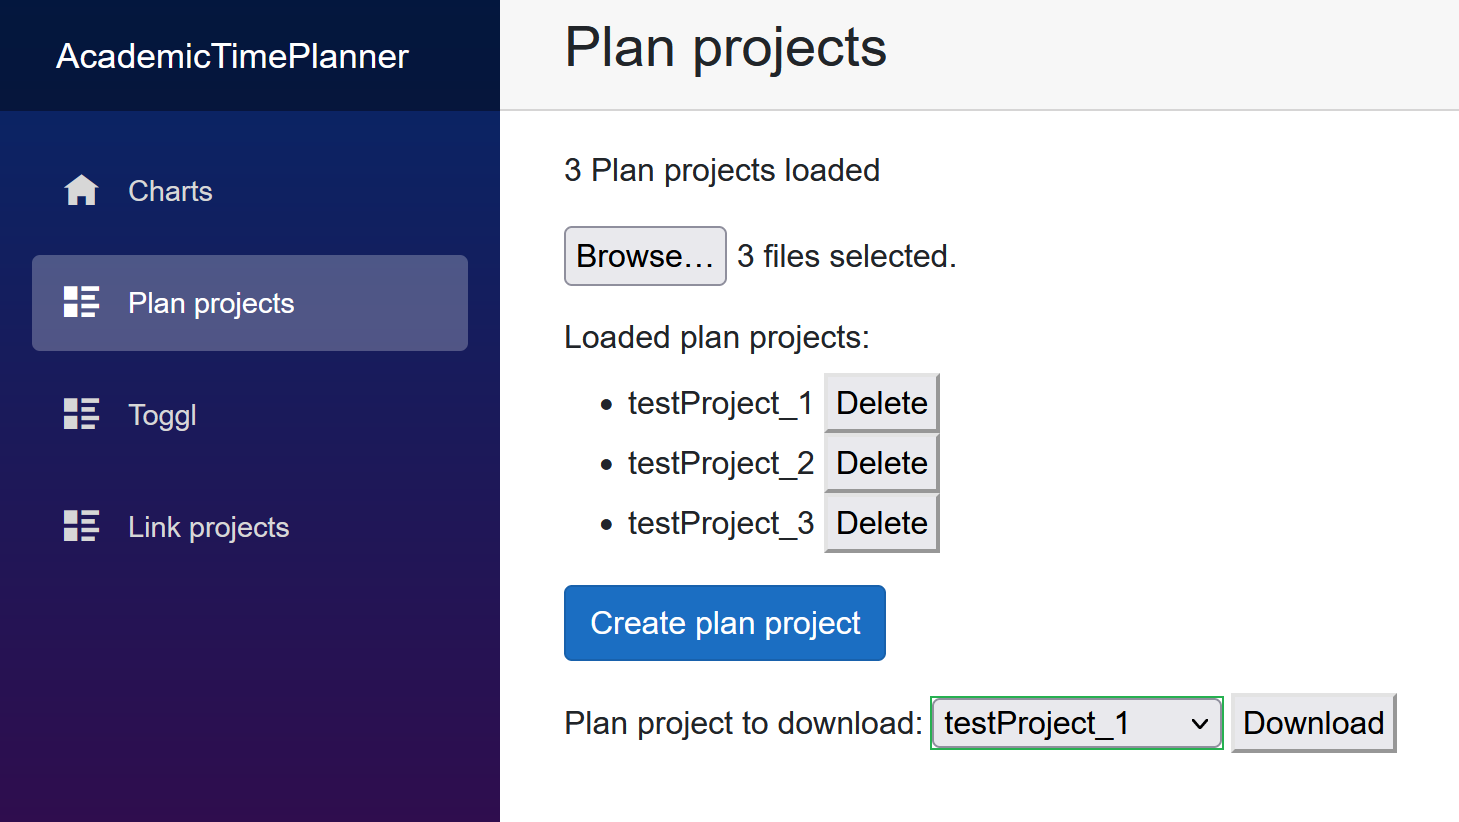
\includegraphics[scale=0.5]{DownloadButton}
	\caption{Download button}
	\label{downloadButton}
\end{figure}

\subsection{Create plan project front-end}
The user has to click on the "Create plan project" button to create a plan project (see figure \ref{createPlanProjectButton}). 
\begin{figure}[H]
	\centering
	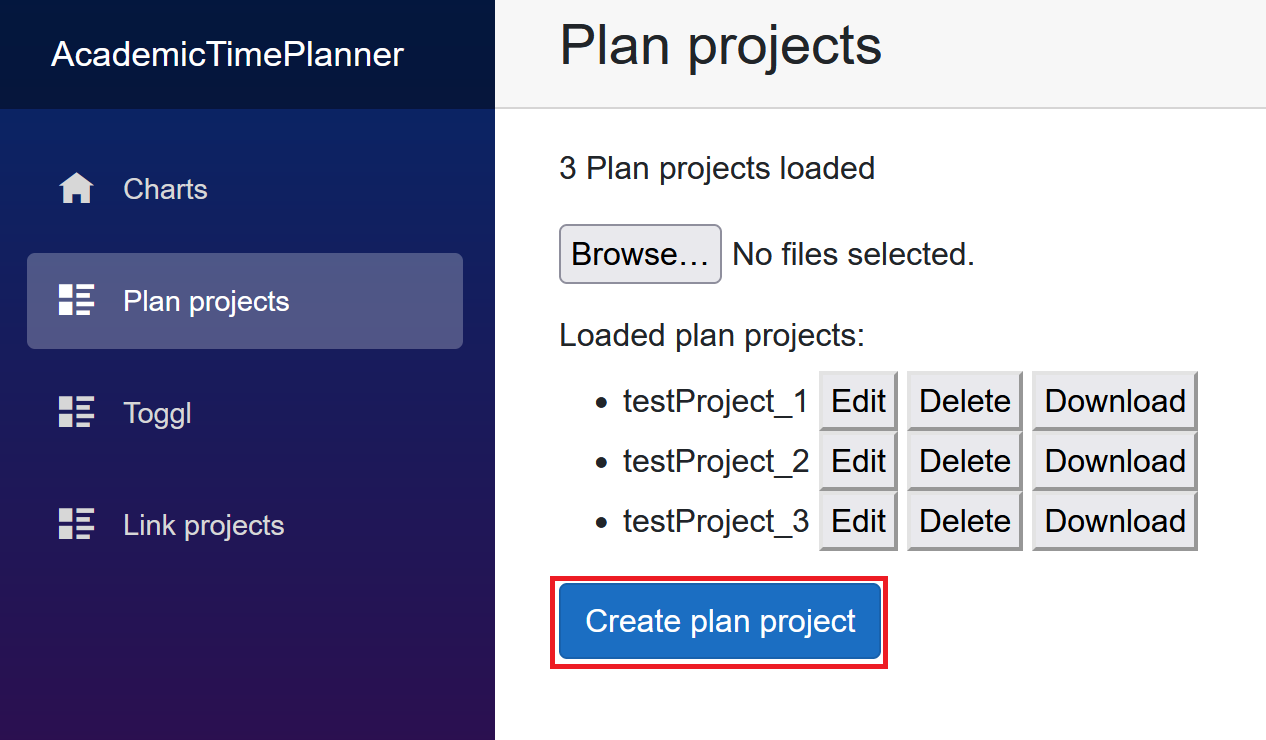
\includegraphics[scale=0.5]{CreatePlanProjectButton}
	\caption{Button to start creating a plan project}
	\label{createPlanProjectButton}
\end{figure}

\subsubsection{Create plan project and plan task}
On the following page the user has to enter the name of the plan project (see figure \ref{createPlanProject}). Not doing so will result in an error on the final overview page before finalizing the project (see figure \ref{createFinalOverviewError}). The next page allows the user to create plan tasks by entering a name and clicking on the "Create task" button (see figure \ref{createPlanTask}). A user can create multiple tasks if desired. This step is optional and the tasks are not needed for the project to function.

\begin{figure}[H]
	\centering
	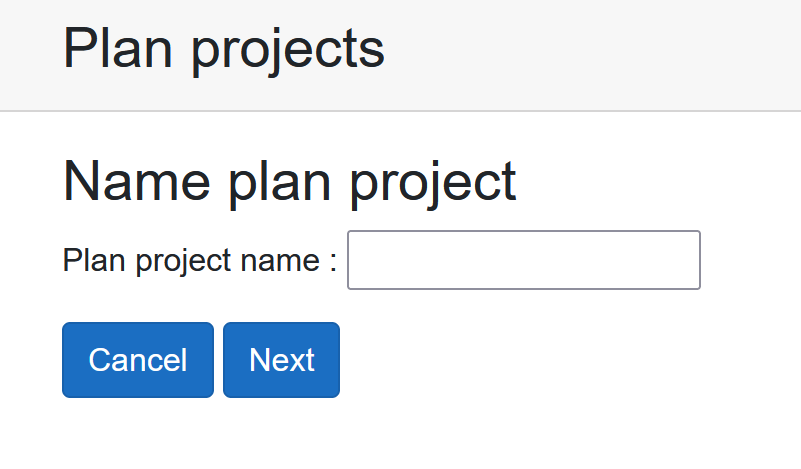
\includegraphics[scale=0.5]{CreatePlanProject}
	\caption{Naming of the plan project}
	\label{createPlanProject}
\end{figure}
\begin{figure}[H]
	\centering
	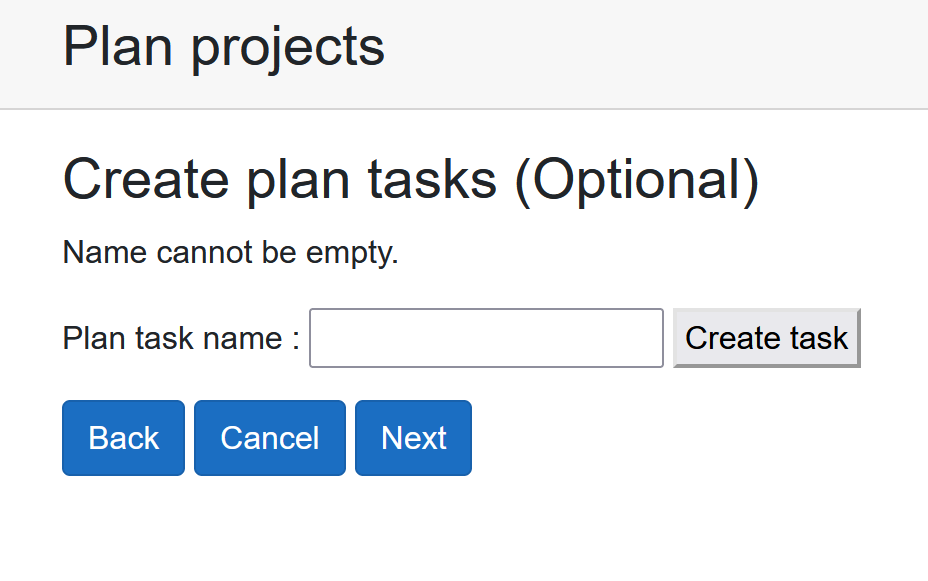
\includegraphics[scale=0.5]{CreatePlanTask}
	\caption{Creating plan tasks}
	\label{createPlanTask}
\end{figure}

\subsubsection{Plan Entries and Plan Entry Repetitions}
On this page the user can choose to create a single plan entry or a plan entry repetition (see figure \ref{createRepetitionOrEntry}). It is possible to create multiples of both and they can be mixed.
\begin{figure}[H]
	\centering
	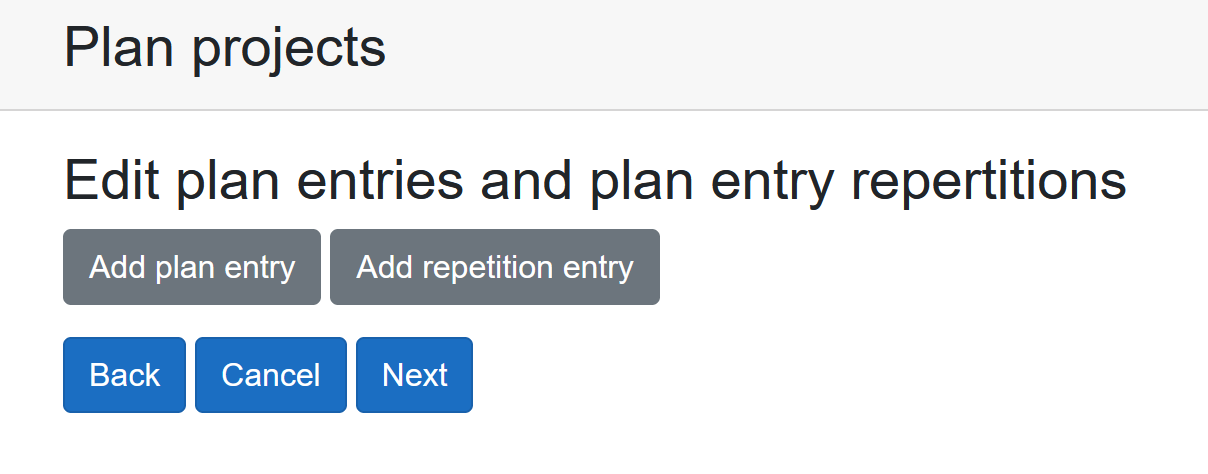
\includegraphics[scale=0.5]{CreateRepetitionOrEntry}
	\caption{Choosing if a single plan entry or a repetition entry should be created}
	\label{createRepetitionOrEntry}
\end{figure}
To create a plan entry all the listed criteria (see figure \ref{createPlanEntry}) have to be met otherwise the create plan entry button will not create a plan entry. If plan tasks were created earlier, a task can be linked to the entry. This step is optional as well. All created plan entries are listed in a list and can be deleted if needed (see figure \ref{createPlanEntry_List}). After creating a plan entry the user can either create another one or click "Next" to save them and go to the previous page to either create repetition entries, go to finalize or to go back and create tasks.
\begin{figure}[H]
	\centering
	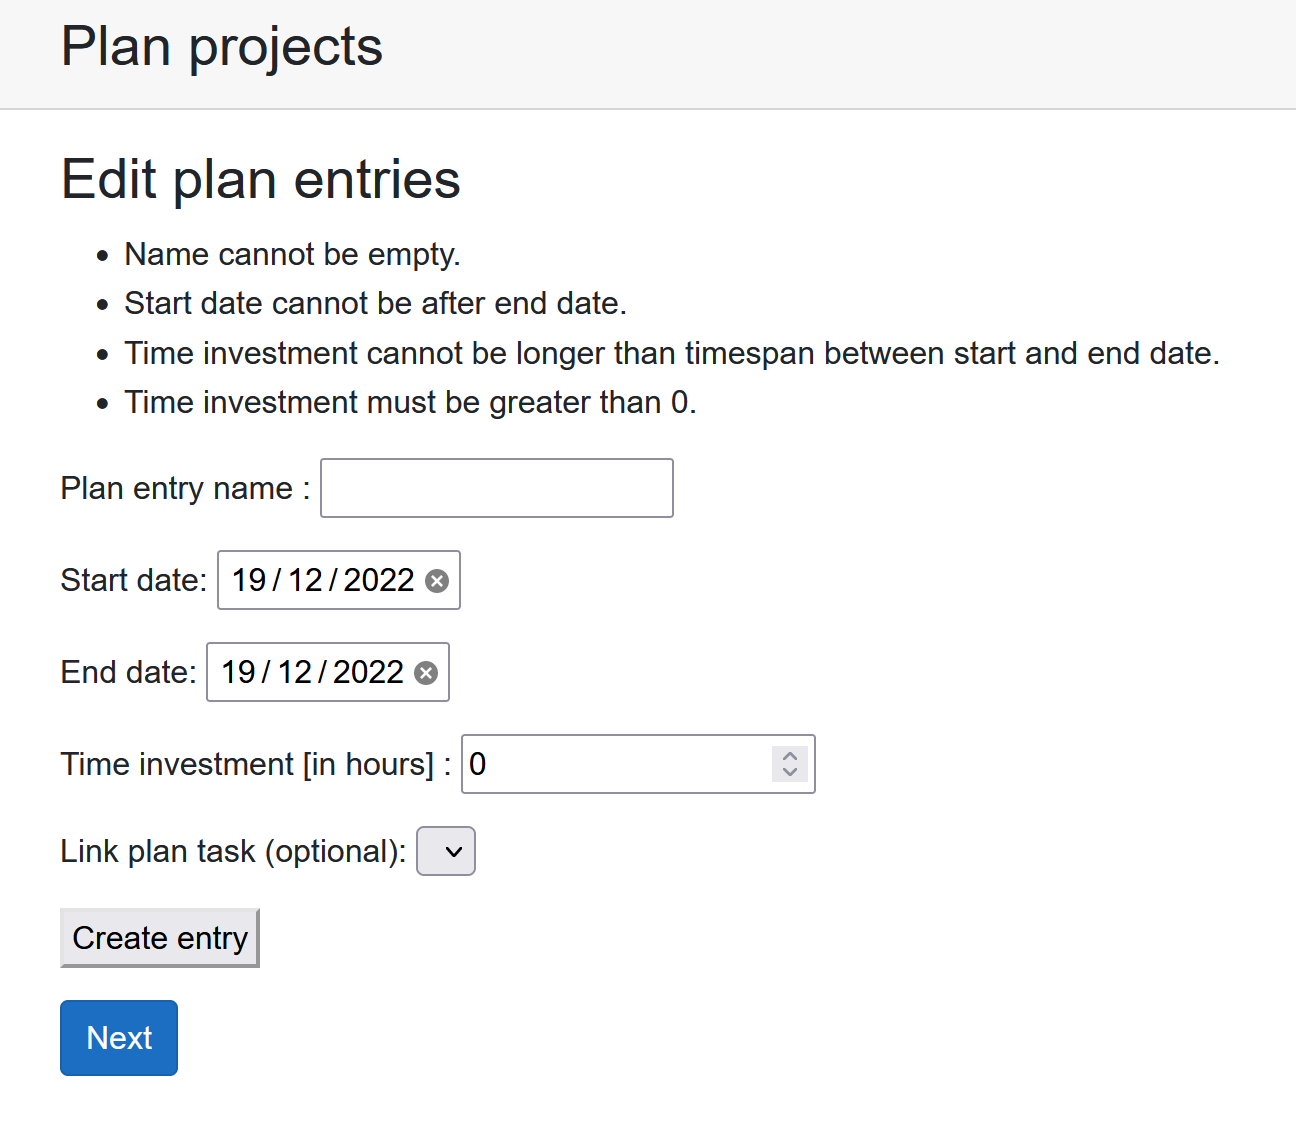
\includegraphics[scale=0.5]{CreatePlanEntry}
	\caption{Creating a plan entry}
	\label{createPlanEntry}
\end{figure}
\begin{figure}[H]
	\centering
	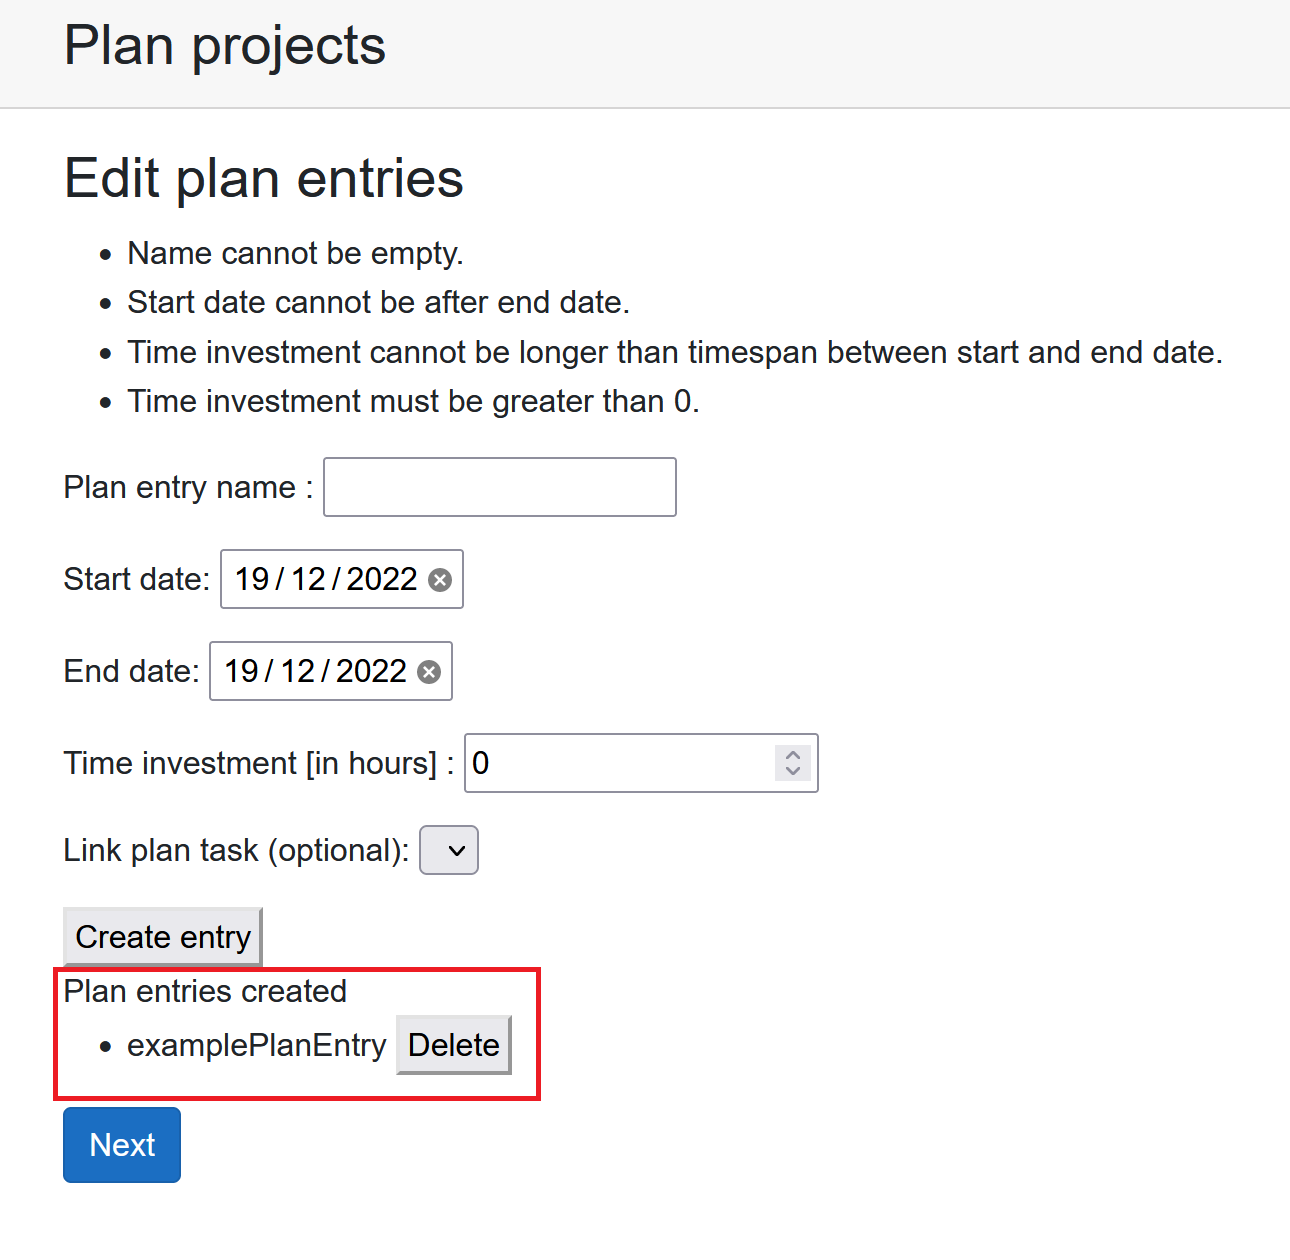
\includegraphics[scale=0.5]{CreatePlanEntry_List}
	\caption{List of created plan entries}
	\label{createPlanEntry_List}
\end{figure}
The creation of a plan entry repetition works similar to the creation of a plan entry. It creates multiple plan entries that repeat after a given interval. The time investment will be distributed evenly over the whole interval by default. If this is not desired then a time span can be entered which starts at the start of an interval. All criteria are listed for the user to check (see \ref{createRepetitionEntry}).
\begin{figure}[H]
	\centering
	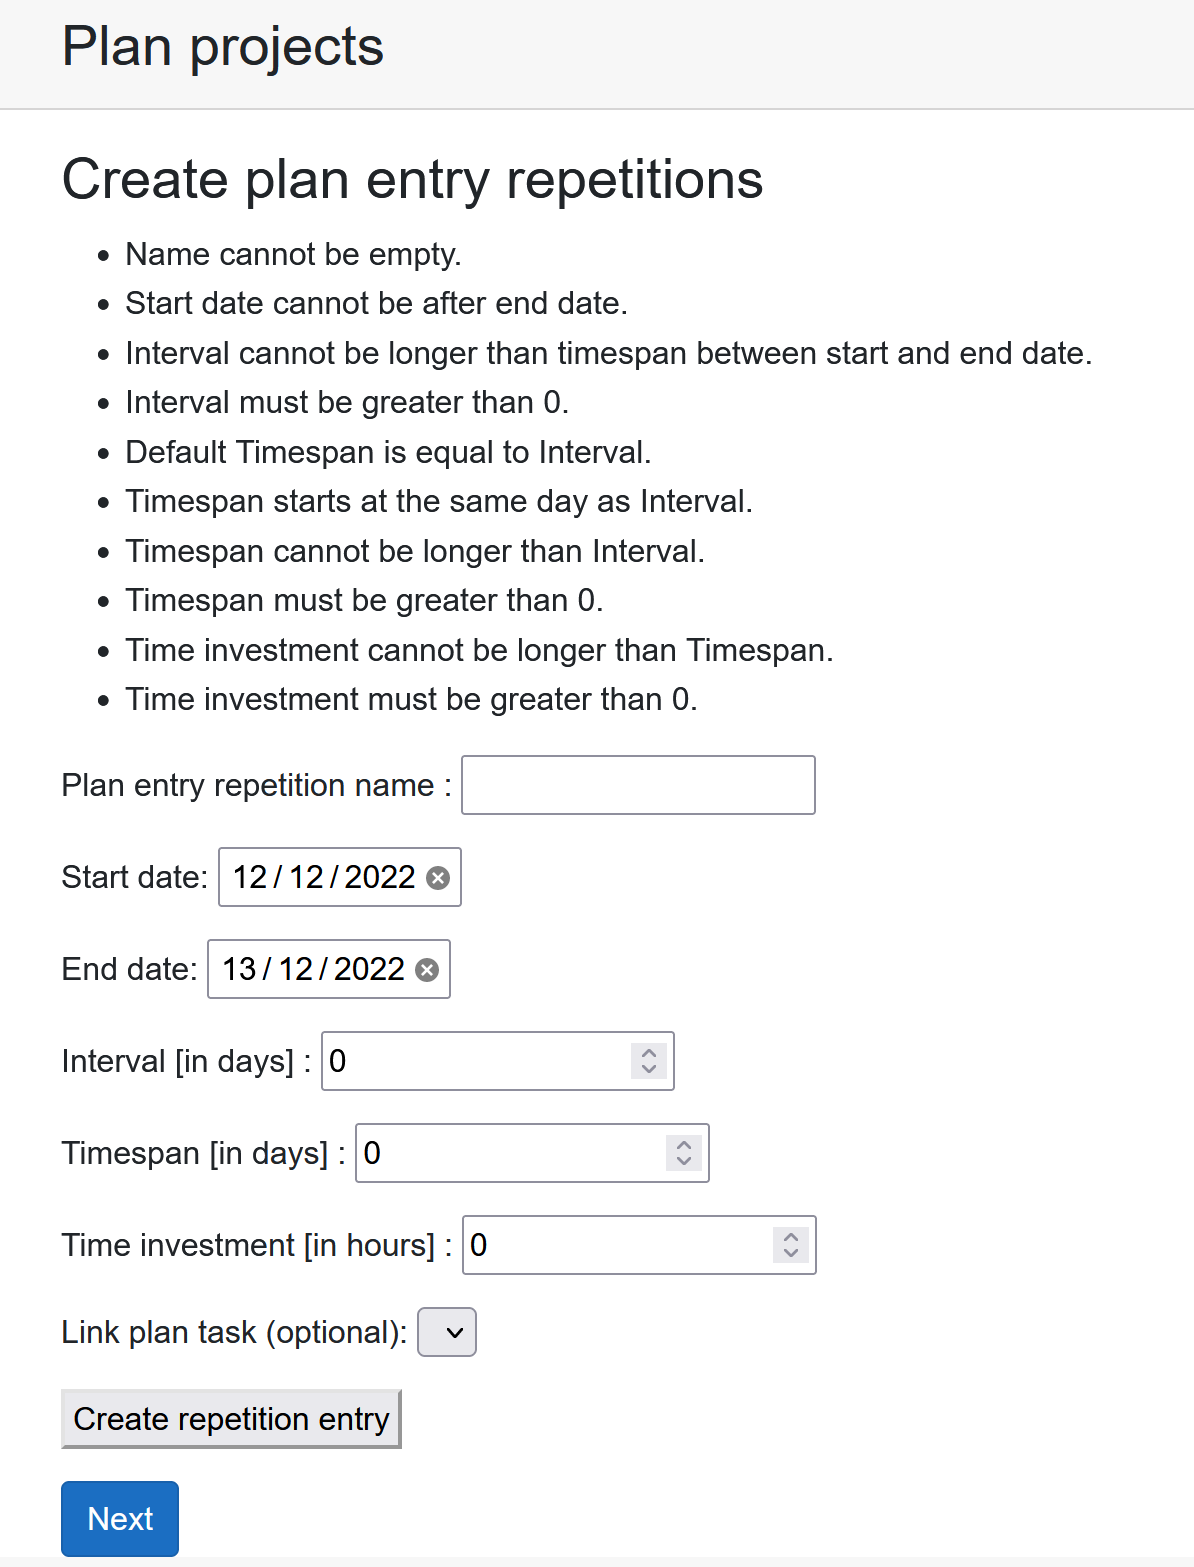
\includegraphics[scale=0.5]{CreateRepetitionEntry}
	\caption{Creating a plan entry repetition}
	\label{createRepetitionEntry}
\end{figure}

\subsubsection{Final overview}
On this last page the user can check if all the tasks, plan entries and repetition entries were created (see \ref{createFinalOverview}). If not, the user can go back and create them and in the case of the previously mentioned missing plan project name the aforementioned error will show (see figure \ref{createFinalOverviewError}). If everything is in order, the user can click on "Finish" to create the plan project and will be brought back to the initial overview of the projects where the newly created project will be added to the list (see figure \ref{loadedPlanProjects}).
\begin{figure}[H]
	\centering
	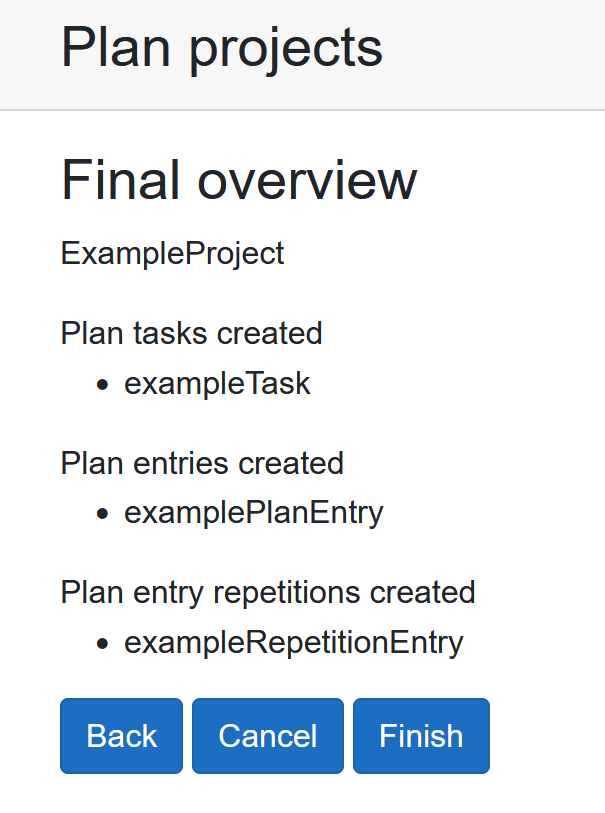
\includegraphics[scale=0.5]{CreateFinalOverview}
	\caption{Final overview of the plan project}
	\label{createFinalOverview}
\end{figure}
\begin{figure}[H]
	\centering
	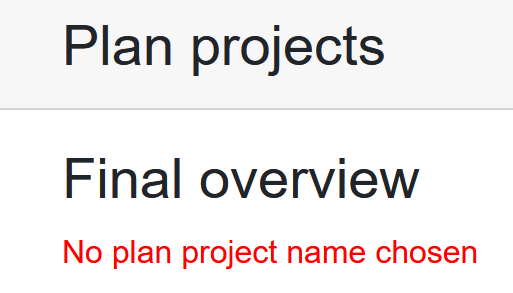
\includegraphics[scale=0.5]{CreateFinalOverviewError}
	\caption{Error message if the plan project was not named}
	\label{createFinalOverviewError}
\end{figure}

\subsection{Edit plan project front-end}
To edit a plan project the user can click on the "Edit" button next to a project in the list (see \ref{editButton}). This will open a similar view as the "Create plan project" button. The only difference being that all the data of the plan project are already entered.
\begin{figure}[H]
	\centering
	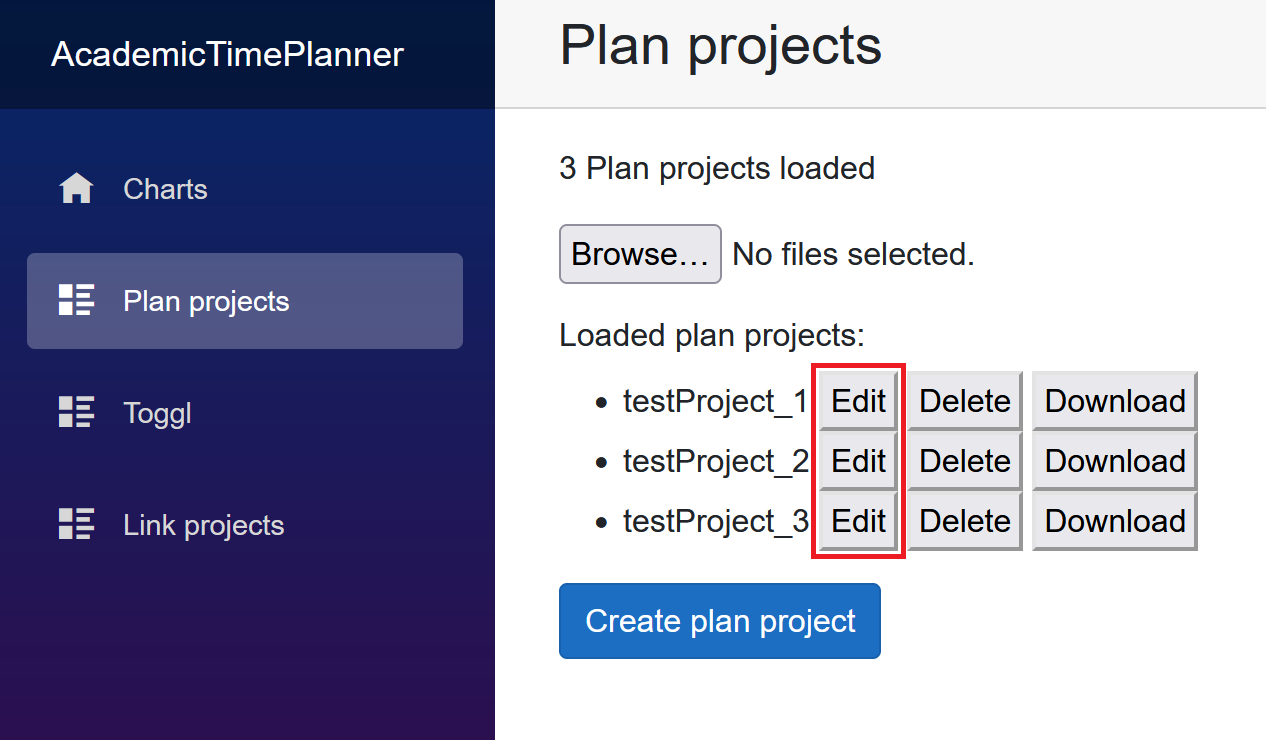
\includegraphics[scale=0.5]{EditButton}
	\caption{Button to start editing process of a plan project}
	\label{editButton}
\end{figure}

\section{Linking of plan projects and Toggl projects} \label{Linking}
The linking page lists the plan projects and the Toggl projects that are present in the ATP as radio buttons. In order to link a Toggl project to a plan project, the user has to select the two and click on "Link projects". An overview of the projects that have already been linked is displayed below the buttons (see figure \ref{Linking init}). It is possible to link the same Toggl project to different plan projects. It is also possible to link multiple Toggl projects to one single plan project. To do this the user just has to select the same plan project once again and link it to the Toggl project of their choice (see figure \ref{Linking multiple}).

\begin{figure}[H]
	\centering
	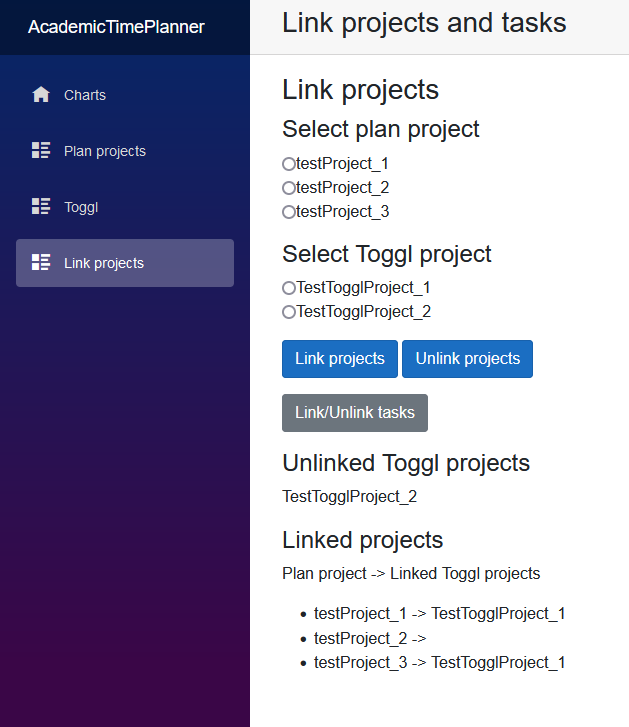
\includegraphics[scale=0.75]{Linking_1}
	\caption{Linking page}
	\label{Linking init}
\end{figure}

\begin{figure}[H]
	\centering
	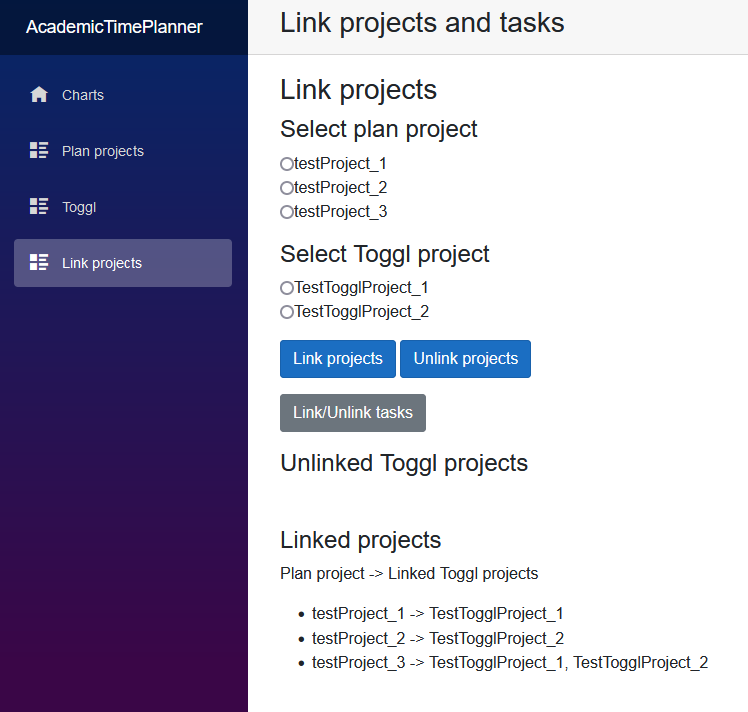
\includegraphics[scale=0.75]{Linking_2}
	\caption{Linking page with multiple Toggl projects linked to one plan project}
	\label{Linking multiple}
\end{figure}

In order to link plan tasks of a plan project to Toggl tasks of the associated Toggl project(s) the user has to click on "Link tasks" which opens up the according submenu which looks similar to the project linking menu and works in just the same way (see figure \ref{Linking tasks init}). In the overview of the linked tasks the Toggl project to which a Toggl task belongs is indicated in brackets. Again, it is possible to link multiple Toggl tasks to one single plan task (see figure \ref{Linking tasks multiple}) and also to link one Toggl tasks to different plan tasks. By clicking on "Link projects" the user can switch back to the project linking menu.

\begin{figure}[H]
	\centering
	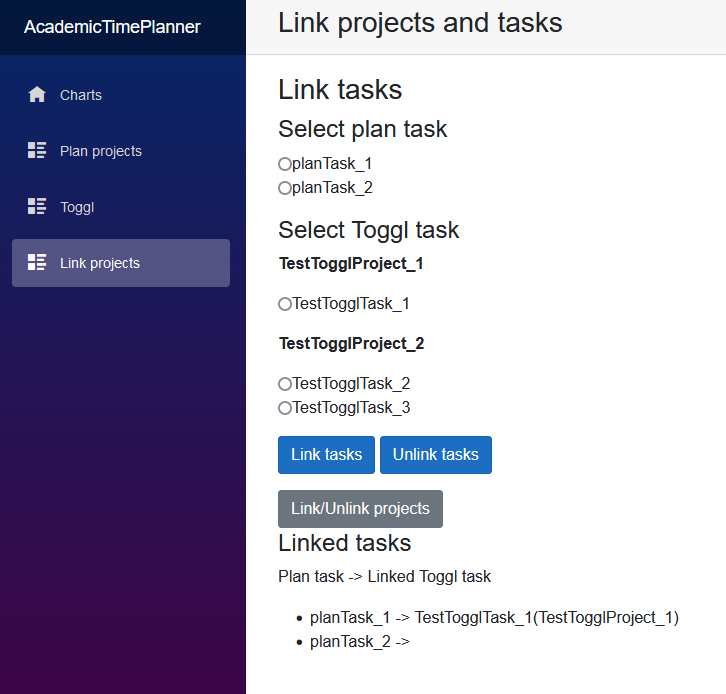
\includegraphics[scale=0.75]{Linking_tasks1}
	\caption{Task linking}
	\label{Linking tasks init}
\end{figure}

\begin{figure}[H]
	\centering
	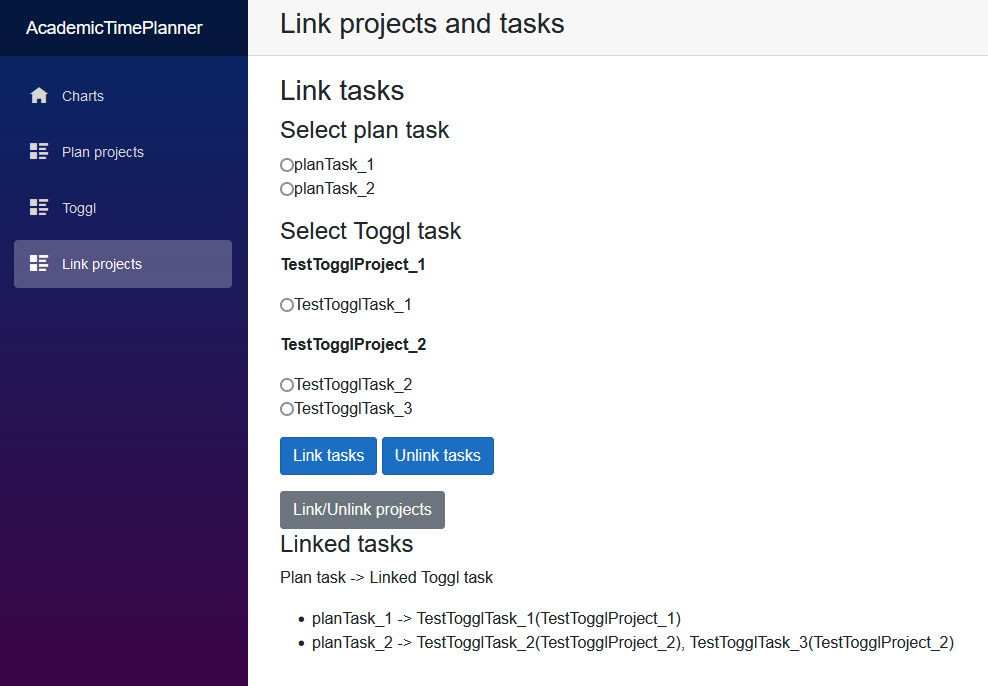
\includegraphics[scale=0.75]{Linking_tasks2}
	\caption{Task linking with multiple Toggl tasks linked to one plan task}
	\label{Linking tasks multiple}
\end{figure}

\section{Concurrent behavior}
In case multiple tabs are opened the application behavior is conservative. This means that if two tabs are opened and a plan project is deleted in one of them while being edited in the other one, finishing the edit after deletion saves the edited project. Therefore, it will be present again in the first tab after reload.

\chapter{Discussion and prospects}
%%% Local Variables:
%%% mode: latex
%%% TeX-master: "../doc"
%%% coding: utf-8
%%% End:
% !TEX TS-program = pdflatexmk
% !TEX encoding = UTF-8 Unicode
% !TEX root = ../doc.tex

In this chapter the approaches and methods applied are discussed. Apart from that, the goals set in chapter \ref{Definition} are reflected and possible prospects are shown.

\section{Discussion}
In this chapter the approaches and methods applied during realization of the project are discussed.

\subsection{Use of Blazor and Fluxor}
Since the application should work platform-independently and other implementation approaches like Java desktop apps or pure web apps were not deemed to be suitable Blazor seemed a fitting choice. Implementation was made easy with documentation provided by Microsoft, most of it concise. Fluxor, on the other hand, did not appear to be very intuitive at first glance. However, it provides an elegant way of front-end behavior control as well as a clear separation between synchronous and asynchronous code. In the light of this the combined use of these two frameworks was deemed appropriate for the realization of the ATP.

\subsection{Use of Plotly.Blazor}
Whereas the documentation of Plotly.Blazor was rather minimalistic, the documentation of Plotly for other languages like Python was quite extensive and thus allowed for implementing the charts display as needed. Apart from that, the amount of code needed for the charts display could be kept at a minimum compared to other packages providing chart components (see chapter \ref{Charts}). Even more complex use cases like the combination of stacked and grouped bar charts could be simulated by clever arrangement of the functionalities provided. Therefore, Plotly.Blazor is a very suitable choice for this application.

\subsection{Application of reduced Scrum methodology}
Applying the two week sprint approach was especially helpful at the beginning of the project allowing for more accurate planning of the different tasks. However, as the project went on the four milestones defined at the beginning became more important than the biweekly sprint plan. What is more, most elements of the Scrum methodology were redundant since the project team consisted of only two persons and one supervisor. In view of this, Scrum does not seem to be applicable to this kind of project. Milestones would be sufficient and can be divided into sub-milestones, if needed.

\subsection{Time planning}
Generally, the planned schedule (see chapter \ref{Time management}) could be kept. The only exception was with milestone \#3 (application status display) where the end was postponed from the Friday to the following Monday due to work for other lectures. The weekly meetings with Mr. Feisthammel were sometimes moved from Tuesday to Wednesday morning due to scheduling issues; this did not impact the progress of the project as we had lectures until 9.00 p.m. on Tuesdays and therefore work on the project continued usually on Wednesday mornings.

\section{Reflection on project goals}
Compared to the definition of the project (see chapter \ref{Definition}) all project goals defined at the beginning have been fulfilled. The Blazor application runs locally in the browser. Planning data is managed by means of ATP plan projects which can be imported, exported and newly created using the user interface of the application. It is also possible to synchronize the Toggl data by fetching the tracked time data from Toggl Track. The last time of synchronization as well as the status of the loaded data are displayed on the user interface. The difference between planned and tracked time data can be read from the charts.

\section{Prospects}
This section describes possible additions and enhancements for the ATP application which might be realized in the future.

\subsection{User experience}
With the standard Blazor input components used so far some parts of the application are awkward to use. For instance, the linking of plan and Toggl projects uses radio buttons instead of checkboxes for the selection of Toggl projects. Therefore, all Toggl projects to be linked to one plan project have to be linked one after another. Moreover, the application looks rather old-fashioned as no CSS rules or other styling improvements have been applied in this prototype. Apart from this, the usability of the application could be enhanced by adding confirmation requests on deletion of plan projects as well as the possibility to remove entries and tasks during creation of a new plan project. Since Blazor input components provide very limited functionality for application handling, an additional package providing more user controls (e.g., Blazorise or Radzen, see chapter \ref{Charts}) might be helpful.

\subsection{Charts}
Currently, the charts only display data on project level. While this is sufficient for small projects, larger ones might not be displayed with adequate accuracy because the different tasks cannot be viewed individually. This could be solved by adding an additional view allowing the separate display of the tasks of a previously selected project.

\subsection{Cross-platform functionality}
In the original prototype cross-platform functionality was enabled by releasing the software on a docker image which could be run on any platform. However, the GitHub Action that had been implemented did not work anymore for the current prototype. Since this feature was not included into the scope of this project it was not given any further consideration. The software currently only runs on Windows and can be downloaded directly from the GitHub project repository. For future versions of the application it is important that the cross-platform functionality is implemented again. The original GitHub action is left in the project repository and may be used as a base.

\subsection{Integration of other time tracking platforms}
As Toggl Track is not the only time tracking platform available and other platforms might be used by students and teachers as well the integration of such platforms is another enhancement to be taken into account. The existing Toggl page could be extended such that users first would have to select the platform before entering their credentials. On the other hand, different platforms use different data formats for tracked time which would require the ATP to wrap the different data formats into one unified format.

\newpage

\addcontentsline{toc}{section}{Table of Figures}
\listoffigures

\addcontentsline{toc}{section}{Bibliography}
\printbibliography[title=Bibliography]
\end{document}